\documentclass[11pt]{article}
\usepackage[T1]{fontenc}
\usepackage{lmodern}
\usepackage[margin=1in]{geometry}
\usepackage{amsmath,amssymb,amsthm,mathtools}
\usepackage{microtype}
\usepackage{enumitem}
\usepackage{tikz}
\usetikzlibrary{arrows.meta,positioning,calc}
\usepackage{xurl}
\usepackage[colorlinks=true,linkcolor=black,citecolor=black,urlcolor=black]{hyperref}
\hypersetup{pdftitle={Uniform Pluricanonical Iitaka Fibrations},pdfauthor={OpenAI}}
\newtheorem{theorem}{Theorem}[section]
\newtheorem{proposition}[theorem]{Proposition}
\newtheorem{lemma}[theorem]{Lemma}
\newtheorem{corollary}[theorem]{Corollary}
\theoremstyle{definition}
\newtheorem{definition}[theorem]{Definition}
\newtheorem{notation}[theorem]{Notation}
\theoremstyle{remark}
\newtheorem{remark}[theorem]{Remark}
\newcommand{\C}{\mathbb C}
\newcommand{\Q}{\mathbb Q}
\newcommand{\Z}{\mathbb Z}
\newcommand{\N}{\mathbb N}
\newcommand{\R}{\mathbb R}
\newcommand{\OO}{\mathcal O}
\newcommand{\PP}{\mathbb P}
\DeclareMathOperator{\Div}{div}
\DeclareMathOperator{\ord}{ord}
\DeclareMathOperator{\vol}{vol}
\DeclareMathOperator{\Supp}{Supp}
\DeclareMathOperator{\Bir}{Bir}
\DeclareMathOperator{\Cl}{Cl}
\DeclareMathOperator{\rk}{rk}
\DeclareMathOperator{\Spec}{Spec}
\DeclareMathOperator{\Hom}{Hom}
\DeclareMathOperator{\End}{End}
\DeclareMathOperator{\tr}{tr}
\DeclareMathOperator{\Pic}{Pic}
\DeclareMathOperator{\Aut}{Aut}
\DeclareMathOperator{\Gal}{Gal}
\setlist{itemsep=2pt,topsep=5pt}
\setcounter{tocdepth}{1}
\numberwithin{equation}{section}
\emergencystretch=1em
\title{Uniform Pluricanonical Iitaka Fibrations}
\author{OpenAI}
\date{October 3, 2026}
\begin{document}
\maketitle
\begin{abstract}
We prove the effective Iitaka fibration conjecture in characteristic zero.
For each dimension, one pluricanonical degree defines the Iitaka fibration
of every smooth integral projective variety of that dimension and nonnegative
Kodaira dimension over an algebraically closed field. The associated sections
generate the full Iitaka function field.
\end{abstract}
\tableofcontents
\section{Introduction}\label{sec:introduction}

For a smooth integral projective variety $X$, the pluricanonical
systems organize the birational information carried by its canonical
divisor. If some $H^0(X,\OO_X(mK_X))$ is nonzero, the maximum of the
dimensions of the resulting rational images is the Kodaira dimension
$\kappa(X)$. In sufficiently large divisible degrees these maps determine
the Iitaka fibration \cite{Iitaka1971}. The question here is whether divisibility and
largeness can be prescribed using only $\dim X$.

To specify the required conclusion, let $K(K_X)\subset k(X)$ be the field
generated by ratios of nonzero sections in the same positive
pluricanonical degree, over all such degrees. This is the function field
of the Iitaka base. A complete system \emph{defines the Iitaka fibration}
if it is nonempty and its section ratios generate $K(K_X)$. Requiring
only an image of dimension $\kappa(X)$ would be weaker: it would allow
a proper finite subfield of the Iitaka field.

\begin{theorem}[Uniform pluricanonical degree]\label{thm:main}
For each integer $d\geq1$ there is an integer $m(d)>0$ such that, over
every algebraically closed field of characteristic zero, the complete
system $|m(d)K_X|$ defines the Iitaka fibration of every smooth integral
projective $d$-fold $X$ with $\kappa(X)\geq0$.
\end{theorem}

Using the log-abundance input from \cite{LA}, this gives an affirmative
resolution of the effective Iitaka fibration conjecture
\cite[Conjecture~1.1]{BirkarZhang2016}. Every positive multiple of
$m(d)$ works as well, by the section-ratio argument in
Section~\ref{sec:completion}.
Thus the same degree works for all nonnegative Kodaira dimensions. In
the general-type case its map is birational. In Kodaira dimension zero
the conclusion is nonemptiness in that degree, with image a point.
The theorem is existential; no small or practical numerical value of
$m(d)$ is asserted.

The proof establishes a second uniform statement at the same time.
A pair in the next theorem is normal and integral; its boundary is
effective and its log canonical divisor is rational Cartier.

\begin{theorem}[Uniform log canonical index]\label{thm:lc-index}
Let $d\geq0$, and let $\Phi\subset[0,1]\cap\Q$ satisfy the descending
chain condition. There is an integer $a(d,\Phi)>0$ such that every
projective log canonical pair $(X,B)$ of dimension $d$, with boundary
coefficients in $\Phi$ and $K_X+B\sim_\Q0$, satisfies
\[
                         a(d,\Phi)(K_X+B)\sim0.
\]
Here the multiple is an integral principal divisor, not merely a
numerically trivial or rationally linearly trivial divisor.
\end{theorem}

\subsection{Context and preceding work}

Effective pluricanonical maps are a quantitative part of birational
classification. The general-type case asks for a uniform birational
degree and was established by Hacon--McKernan, Takayama, and Tsuji
\cite{HaconMcKernan2006,Takayama2006,Tsuji2007}.
Hacon--McKernan--Xu's theorem for big log canonical adjoints permits
boundary coefficients in a fixed DCC set \cite[Theorem~1.3]{HMX2014}.
The lower-Kodaira-dimensional problem has an additional feature:
the general fibre contributes torsion and monodromy data which do not
appear in the big case.

Fujino--Mori obtained a uniform pluricanonical degree for threefolds
of Kodaira dimension one using their canonical bundle formula
\cite[Corollary~6.2]{FujinoMori2000}. Their denominator argument
identifies finite characters on an extended Hodge line and bounds
their orders using the middle Betti number of a canonical cover
\cite[Theorem~3.1 and Sections~3.6--3.8]{FujinoMori2000}.
Viehweg--Zhang obtained effective results for Iitaka bases of dimension
two, with constants controlled by invariants of the general fibre
\cite[Theorem~0.2]{ViehwegZhang2009}. Birkar--Zhang proved a general
effective Iitaka theorem with dependence on the dimension, the least
nonvanishing canonical degree of the general fibre, and a middle Betti
number of a smooth model of its canonical cover
\cite[Theorem~1.2]{BirkarZhang2016}. Their effective birationality theorem
for polarized adjoints is the final effective input used here
\cite[Theorem~1.3]{BirkarZhang2016}. The present argument supplies the
required denominator control without assuming a uniform bound for
those middle Betti numbers.

The index problem has its own inductive structure. Xu relates
zero-boundary klt index bounds to bounds with boundary
\cite[Theorem~1.8]{Xu2019}. Birkar proves the index theorem for rationally
connected klt Calabi--Yau pairs in every fixed dimension
\cite[Corollary~1.8]{Birkar2025}; his boundedness theorem for generalized
Calabi--Yau pairs also controls torsion on rationally connected bases
\cite[Theorem~1.7]{Birkar2025}. We combine these results with an arithmetic
Stein-degree theorem \cite[Main Theorem]{SD} to pass from klt pairs to
normal lc pairs without an index theorem for nonnormal pairs.

\subsection{Inputs and contributions}

One major input must be distinguished from standard minimal-model
technology. We use the good-log-minimal-model theorem of the companion
\emph{Log abundance in characteristic zero}
\cite[Theorem~11.1]{LA}, stated precisely in
Theorem~\ref{thm:good-models}. It includes nonvanishing and is used in
all dimensions. It is not being inferred from finite generation for
big adjoints. The other companion inputs are the chain and tracking
lemmas in \cite{U4}, and the arithmetic Stein-degree bound in \cite{SD}.
The arguments of \cite{R4} provide the preceding fourfold treatment of
relative denominators and rationally connected torsion.

The proof extends the canonical-index method of \cite{U4} to arbitrary
dimension. There are two substantial extensions. First, we prove a
relative denominator bound by decomposing the geometric generic fibre,
degenerating its individual factors, and controlling their volume-form
characters on normal components of a dlt special fibre. This separates
the potentially unbounded ramification of semistable reduction from
the bounded characters that enter the moduli divisor. The argument
uses the absence of horizontal boundary and only lower-dimensional
normal lc index bounds. It is therefore a reusable relative statement,
not merely the final step of the Iitaka theorem.

Second, the small-volume argument in \cite{U4} is extended to Iitaka
bases of arbitrary dimension. Weak positivity supplies a fibre-to-total
volume comparison, while flattening ensures that codimension-two
losses on the base create no divisorial poles on the original smooth
model. This gives scalar bounds for section orders and Seshadri
constants. We then give the dimension-dependent calculations in the
Frobenius diagonal argument and in the compatible-chain argument.
Those constructions are adaptations of \cite{U4}; the new claim is
their use in the all-dimensional induction, not a new origin for the
constructions themselves.

\subsection{The induction}

We prove Theorems~\ref{thm:main} and~\ref{thm:lc-index} simultaneously.
Fix $n$ and suppose both are known in smaller dimensions. The relative
step starts with a contraction $f:X\to Z$ from a klt $n$-fold, with
$\dim Z>0$ and $K_X$ rationally linearly pulled back from $Z$.
The canonical bundle formula writes
\[
                    K_X\sim_{\Q}f^*(K_Z+B_Z+M_Z),
\]
where $B_Z$ is the discriminant divisor and $M_Z$ is the moduli
divisor. Section~\ref{sec:denominators} bounds a Cartier multiple of
the moduli divisor on a birational base model using only
lower-dimensional normal lc indices. When $K_X\sim_{\Q}0$ and the
base has a rationally connected smooth resolution, this denominator
bound combines with torsion control on the base to bound the canonical
index of $X$.

Section~\ref{sec:reductions} then reduces failure of the zero-boundary
klt index bound to terminal varieties $V$ with canonical indices
$r\to\infty$ and countable birational groups. Their canonical cyclic
covers $\pi:Y\to V$ have degree $r$ and deck group $G$. Every
$G$-equivariant rational fibration of $Y$ with positive-dimensional
base and fibre has general-type smooth geometric generic fibre.
We call such fibrations intermediate. The corresponding assertion holds for
intermediate rational fibrations of $V$.

Choose an ample rational Cartier divisor $L$ on $V$ with
$1\le L^n\le2$. For an ample rational Cartier divisor $P$, write
$\varepsilon(P)$ for its very general Seshadri constant: the infimum
of $P\cdot C/\operatorname{mult}_xC$ over integral curves through a
very general point $x$. Section~\ref{sec:scalar} uses lower-dimensional
effective Iitaka fibrations to bound section orders on $V$ and bound
$\varepsilon(L)$ below uniformly. The pullback polarization has
$(\pi^*L)^n=rL^n$.

For $t\ge2$, let $Z_t=Y^t/G_{\mathrm{diag}}$, where $G$ acts by
the same deck transformation in every slot. Let
$\theta_t:Z_t\to V^t$ be the induced finite map and set
$P_t=\theta_t^*(\sum_{i=1}^t\operatorname{pr}_i^*L)$.
Together, the scalar estimates and the diagonal argument of
Section~\ref{sec:diagonal} give
\[
       \varepsilon(\pi^*L)\ge c r^{1/n},
       \qquad \varepsilon(P_t)\le Ct^2,
\]
with $c,C>0$ depending only on $n$. The second bound supplies curves
of bounded $P_t$-degree divided by marked multiplicity.

Section~\ref{sec:transport} arranges these curves into chains compatible
with coordinate projections. The resulting positive-dimensional
leaves project generically finitely onto their images in each
coordinate, and comparison of their projection degrees gives a
degree-one coordinate-forgetting map.
Rational recovery of its missing coordinate turns local flows into
uncountably many birational self-maps of $V$, a contradiction. This
bounds the zero-boundary klt index. The normal lc reduction in
Section~\ref{sec:index} then proves Theorem~\ref{thm:lc-index} in
dimension $n$. Finally, Section~\ref{sec:completion} reuses the
denominator bound with polarized effective birationality to prove
Theorem~\ref{thm:main} in that dimension. Figure~\ref{fig:induction}
records the dependencies after the induction statements have been
formally introduced.

\section{Conventions and the induction hypotheses}\label{sec:preliminaries}

Until the final field-descent argument we work over $\C$. Varieties are
integral and projective unless another setting is stated. We use the
standard discrepancy conventions for klt, dlt, and lc pairs
\cite{Kollar2013}. All boundaries in the proof are rational. A
\emph{rational Cartier divisor} means a $\Q$-Cartier $\Q$-divisor.
Canonical divisors are chosen compatibly when forms are pulled back
or residues are taken. On a normal variety, sections of an integral
Weil divisor always mean sections of its rank-one reflexive divisorial
sheaf.

For rational divisors $D,E$ we write $D\preceq E$ if $E-D$ is rationally
linearly equivalent to an effective divisor. An index bound is a
\emph{common trivializing multiple}: a single integer kills all the
actual divisor classes under consideration and clears their
coefficients. A bound on the least possible integers implies a common
multiple by taking their least common multiple.

A \emph{contraction} is a projective surjective morphism
$f:X\to Z$ of normal varieties such that $f_*\OO_X=\OO_Z$. Its generic
fibre is geometrically integral in characteristic zero. A rational
fibration is understood through a relatively algebraically closed
subfield of the total function field; after resolution and Stein
factorization it has connected fibres. A smooth geometric generic
model is a smooth projective model of the geometric generic fibre.

For generalized pairs, the nef data consist of a nef rational Cartier
divisor on a higher birational model, together with its compatible
pullbacks. A moduli b-divisor is \emph{b-nef and b-Cartier} if it is the
Cartier closure of a nef divisor on one such model. The generalized
discrepancies are computed by pulling back the full adjoint, including
these nef data. We use the conventions of \cite{BirkarZhang2016}.

\begin{theorem}[Good minimal models; \cite{LA}]
\label{thm:good-models}
Let $(X,B)$ be a projective lc pair over $\C$ with effective rational
boundary and pseudo-effective $K_X+B$. Then $(X,B)$ has a good log
minimal model. In particular, its adjoint is nonvanishing, and on the
good model the adjoint is semiample.
\end{theorem}

This is the rational-boundary case of \cite[Theorem~11.1]{LA}.
We also use the standard klt MMP and its discrepancy comparisons
\cite{BCHM2010}. For klt pairs with a good minimal model, an MMP with
scaling can be chosen terminating at such a model. We will specify
relative or equivariant uses when they arise; they do not require a
separate unmentioned abundance assumption.

\begin{notation}[Induction statements]\label{not:induction}
Let $I_n$ denote Theorem~\ref{thm:main} in dimension $n$, and let $L_n$
denote Theorem~\ref{thm:lc-index} in dimension $n$, for every rational
DCC coefficient set. Let $K_n$ denote its zero-boundary klt case:
there is a common integer $a_n>0$ with $a_nK_X\sim0$ for all projective
klt $n$-folds satisfying $K_X\sim_\Q0$.
\end{notation}

The dimension-zero statements hold with degree one. In a fixed
induction step we assume $I_j,L_j$ for all $j<n$. By global ACC
\cite[Theorem~1.5]{HMX2014}, the coefficients of numerically trivial
lc pairs of fixed dimension with coefficients in a fixed DCC set
belong to a finite subset. Thus proving $L_n$ for every finite
rational coefficient set proves its stated DCC form. This observation
also applies to the different coefficients that occur in adjunction.

The dependency diagram below distinguishes $K_n$ from $L_n$. In
particular, the proof of the moduli denominator uses only $L_j$ with
$j<n$, not the dimension-$n$ index statement being established.
\begin{figure}[htbp]
\centering
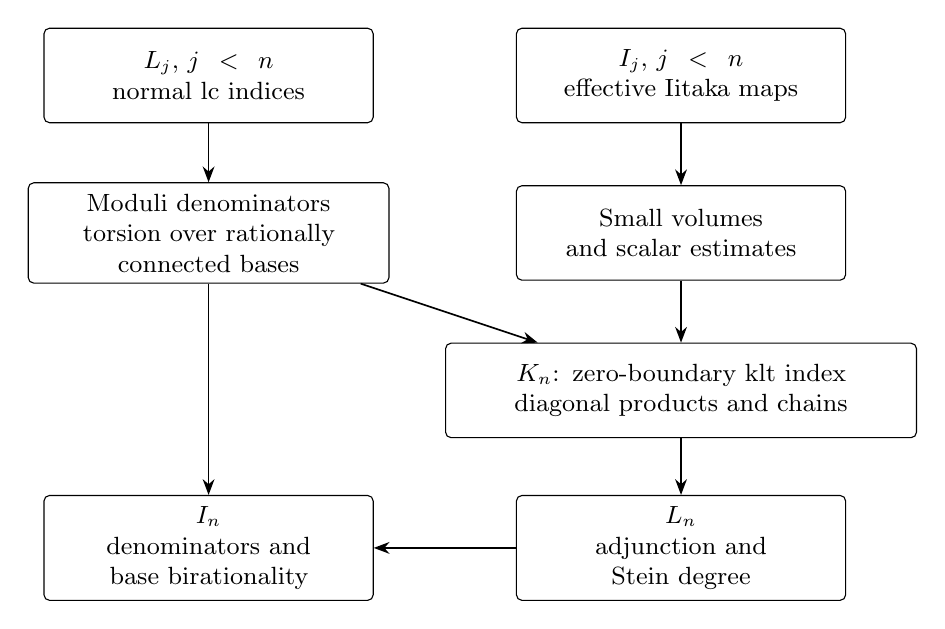
\begin{tikzpicture}[
 box/.style={draw,rounded corners=2pt,align=center,font=\small,
             text width=39mm,minimum height=12mm,inner sep=4pt},
 arr/.style={-{Stealth[length=2mm]},semithick}]
\node[box] (lowL) at (0,0) {$L_j$, $j<n$\\normal lc indices};
\node[box] (lowI) at (6,0) {$I_j$, $j<n$\\effective Iitaka maps};
\node[box,text width=43mm] (den) at (0,-2) {Moduli denominators\\torsion over rationally\\connected bases};
\node[box] (scalar) at (6,-2) {Small volumes\\and scalar estimates};
\node[box,text width=57mm] (idx) at (6,-4) {$K_n$: zero-boundary klt index\\diagonal products and chains};
\node[box] (lc) at (6,-6) {$L_n$\\adjunction and Stein degree};
\node[box] (iit) at (0,-6) {$I_n$\\denominators and base birationality};
\draw[arr] (lowL)--(den);
\draw[arr] (lowI)--(scalar);
\draw[arr] (den)--(idx);
\draw[arr] (scalar)--(idx);
\draw[arr] (idx)--(lc);
\draw[arr] (lc)--(iit);
\draw[arr] (den)--(iit);
\end{tikzpicture}
\caption{One induction step. The left-hand route supplies the relative
index control used in reducing $K_n$; the right-hand route supplies its
section-order estimates. After $K_n$ is proved, adjunction and Stein
degree give $L_n$, and the denominator bound also feeds the final
proof of $I_n$, as shown by the direct left-hand arrow. Arrows record
the main dependencies, not morphisms of
varieties.}\label{fig:induction}
\end{figure}


\subsection{Geometric generic fibres and fields of definition}

All finite collections of varieties, maps, divisors, and rational
forms can be defined over a finitely generated field of characteristic
zero. Algebraically closed extensions preserve the singularity
conditions, dimensions of section spaces, Cartierness, and triviality
of the line bundles used here. For singularities one may spread a log
resolution and its discrepancy calculation; for sections and
trivializations one uses flat base change and faithful flatness.
Consequently the induction hypotheses apply to geometric generic
fibres, by comparison with an algebraically closed field embedded in
$\C$.

We occasionally need very general points to satisfy countably many
section-order conditions simultaneously. One may make these choices
over $\C$, or use points geometric generic over a countable field of
definition for the varieties and all the systems involved. Moving
members below are taken at geometric generic parameters. Dominant
extensions needed to define models or maps do not specialize a
previously chosen generic parameter.

We record one descent observation used repeatedly. If $F$ is a
geometrically integral normal projective variety over a field $K$
and a given reflexive pluricanonical sheaf becomes the trivial line
bundle over $\overline K$, then it is already a line bundle over $K$
and is trivial there. Local freeness descends faithfully flatly.
Base change identifies its space of sections with a one-dimensional
space after extension, and any nonzero section over $K$ becomes a
generator, hence is a generator before extension as well. The same
argument applies to a specified integral log pluricanonical divisor.

\section{Normal log canonical indices and finite covers}\label{sec:index}

Two preliminary arguments will keep the induction within normal varieties.
The first recovers an lc index from the index of one normalized boundary
component and its Stein degree. The second separates finite actions on
the factors of a quasi-\'etale product cover. Throughout this section,
the inductive assertions $I_j,L_j$ are available for $j<n$; the assertion
$K_n$ is used only in Proposition~\ref{prop:lc-reduction}.

\subsection{Descent from a normalized boundary component}

We begin with an elementary descent observation. A rational
$q$-canonical form means a nonzero rational section of the $q$th tensor
power of the canonical line at the generic point. Its divisor is defined
on a normal variety by orders at prime divisors.

\begin{lemma}[Descent of a vertical principal divisor]\label{lem:vertical-descent}
Let $f:X\to Z$ be a contraction of normal projective varieties over a
field of characteristic zero. A rational function on $X$ whose divisor
has no horizontal component belongs to the subfield $k(Z)\subset k(X)$.
Suppose, in addition, that $(X,B)$ is a rational pair with
$K_X+B\sim_{\Q}0$, and that $q(K_{X_\eta}+B_\eta)\sim0$ on the generic
fibre. There are a rational $q$-canonical form $s$ and a rational Cartier
divisor $D\sim_{\Q}0$ on $Z$ such that
\begin{equation}\label{eq:index-vertical-form}
                 \Div(s)+qB=f^*D.
\end{equation}
\end{lemma}

\begin{proof}
The generic fibre $X_\eta$ is normal and projective, with
$H^0(X_\eta,\OO_{X_\eta})=k(Z)$. A rational function with vertical
divisor restricts to a function with neither zeros nor poles at any
prime divisor of $X_\eta$. Normality makes it regular, and hence a
member of $k(Z)$.

For the second assertion, extend a trivializing rational form on
$X_\eta$ to a rational $q$-canonical form $s$ on $X$, using any rational
top form on $Z$ to identify relative and absolute canonical lines.
The divisor $H=\Div(s)+qB$ is vertical. Choose $a>0$ and a rational
$aq$-canonical form $\tau$ with $\Div(\tau)+aqB=0$. The function
$s^{\otimes a}/\tau$ has divisor $aH$, so the first assertion writes
it as $f^*h$ for some $h\in k(Z)^*$. Thus
$H=f^*((1/a)\Div(h))$, as required.
\end{proof}

\begin{proposition}[Reduction to the zero-boundary klt index]\label{prop:lc-reduction}
Assume $L_j$ for every $j<n$ and $K_n$. Then $L_n$ holds: for every
finite set $\Gamma\subset[0,1]\cap\Q$ there is an integer
$c(n,\Gamma)>0$ such that
\[
                    c(n,\Gamma)(K_X+B)\sim0
\]
for every normal projective lc $n$-fold pair $(X,B)$ with coefficients
in $\Gamma$ and $K_X+B\sim_{\Q}0$.
\end{proposition}

\begin{proof}
The assumptions give the zero-boundary klt index bounds through
dimension $n$. Xu's klt induction theorem
\cite[Theorem~1.8]{Xu2019} therefore supplies the assertion when $(X,B)$
is klt. We prove the non-klt case without an slc index statement.

\emph{A Mori fibre space and a horizontal lc divisor.}
Take a crepant $\Q$-factorial dlt modification, and enlarge $\Gamma$
by $1$. Write $T=\lfloor B\rfloor\ne0$. For sufficiently small
rational $\epsilon>0$, the pair $(X,B-\epsilon T)$ is klt and
\[
                  K_X+B-\epsilon T\sim_{\Q}-\epsilon T
\]
is not pseudo-effective: its intersection with the $(n-1)$st power
of an ample divisor is negative. The klt minimal model program
\cite[Corollary~1.3.3]{BCHM2010} ends in a Mori fibre space
$f:X'\to Z$.

The full log canonical divisor remains crepant through this program.
Indeed, fix compatible canonical divisors and write
$r(K_X+B)=\Div(h)$. Divisorial contractions push forward this same
identity, and flips preserve it under their codimension-one
identification. On a common resolution, both pullbacks equal
$r^{-1}\Div(h)$. Thus the full pairs on all models are lc, even
though they need not be dlt. The exact order of their log canonical
divisors is unchanged. We henceforth write $(X,B)$ for the last
model.

If $\dim Z=0$, the klt log Fano pair $(X,B-\epsilon T)$ shows that
$X$ is of Fano type. The bounded complement theorem
\cite[Theorem~1.7]{Birkar2019}, with a fixed hyperstandard set containing
$\Gamma$, gives a bounded integer $c$ and a complement $B^+\ge B$
with $c(K_X+B^+)\sim0$. The effective divisor $B^+-B$ is numerically
trivial, hence zero by intersection with an ample class. This settles
that case.

Suppose $\dim Z>0$. On the Mori fibre space the surviving transform
of $T$ is relatively ample, since $\epsilon T$ is relatively
$\Q$-linearly equivalent to $-(K_X+B-\epsilon T)$. In particular,
some prime component $S$ of $T$ dominates $Z$. Let
$\nu:S^\nu\to S$ be its normalization. Divisorial adjunction gives
\begin{equation}\label{eq:index-adjunction}
             (K_X+B)|_{S^\nu}=K_{S^\nu}+\Theta.
\end{equation}
Here $(S^\nu,\Theta)$ is a normal lc pair and $\Theta$ is effective;
its coefficients belong to the rational DCC set of differents
determined by $\Gamma$ \cite{KollarMori1998}. Its adjoint is
$\Q$-linearly trivial. The lower-dimensional assertion $L_{n-1}$,
together with global ACC as in the conventions, therefore bounds a
trivializing multiple of $K_{S^\nu}+\Theta$.

\emph{A common form degree.}
The geometric generic fibre of $f$ is a normal projective lc pair
of dimension less than $n$, with the same coefficient set. The
assertions $L_j$, $j<n$, bound a trivializing multiple there, and
linear triviality descends in that same degree to $k(Z)$. To see the
last point, the corresponding divisorial sheaf becomes an invertible
trivial sheaf after algebraic closure. Invertibility descends
faithfully flatly. Flat base change for global sections then gives
a one-dimensional space over $k(Z)$, and its evaluation map is an
isomorphism because it becomes one after the field extension.

Choose a common integer $q$, depending only on $n$ and $\Gamma$,
which clears $\Gamma$ and trivializes both this fibre adjoint and
$K_{S^\nu}+\Theta$. Lemma~\ref{lem:vertical-descent} gives
\eqref{eq:index-vertical-form}, with $D\sim_{\Q}0$. At the generic
point of $S$, the form $s$ has precisely its logarithmic pole of
order $q$. Its $q$-fold residue is a nonzero rational
$q$-canonical form $v$ on $S^\nu$, and adjunction gives the equality
of actual divisors
\begin{equation}\label{eq:index-residue-divisor}
       \Div(v)+q\Theta=(f\circ\nu)^*D.
\end{equation}
For this equality one may first take a sufficiently divisible
tensor power and apply the usual pluricanonical adjunction
isomorphism; dividing the resulting equality of divisorial orders
gives \eqref{eq:index-residue-divisor}. No Cartier assumption in
degree $q$ along the whole of $S$ is needed.

\emph{Stein factorization and norm.}
Choose a trivializing $q$-log canonical form $v_0$ on
$(S^\nu,\Theta)$. Then $a=v/v_0\in k(S)^*$ satisfies
\[
                     \Div(a)=(f\circ\nu)^*D.
\]
Factor the map as $S^\nu\xrightarrow{g}Y\xrightarrow{h}Z$, where
$g$ is a contraction and $h$ is finite, with $Y$ normal. The first
part of Lemma~\ref{lem:vertical-descent} gives $a\in k(Y)^*$.
Injectivity of pullback for rational Cartier divisors under the
surjective map $g$ yields
\[
                          h^*D=\Div_Y(a).
\]
One can check this injectivity at a prime divisor of $Y$, where a
nonzero order remains nonzero at a prime divisor above it. The norm
identity for the finite morphism $h$ now gives
\begin{equation}\label{eq:index-norm}
       (\deg h)D=\Div_Z\bigl(N_{k(Y)/k(Z)}a\bigr).
\end{equation}

It remains to bound $\deg h$, not the degree of any gluing cover.
Apply the arithmetic Stein-degree theorem \cite[Theorem~1.1]{SD}
to $(X_\eta,B_\eta)$ over $k(Z)$, with its prime coefficient-one
divisor $S_\eta$ and parameter $t=1$. This fibre is normal,
integral and projective, and its field of global functions is
$k(Z)$. The relative algebraic closure of $k(Z)$ in $k(S_\eta)$
is exactly $k(Y)$. Hence $\deg h$ is bounded in terms of the fibre
dimension, and therefore in terms of $n$.

Equations~\eqref{eq:index-vertical-form} and \eqref{eq:index-norm}
show that $q(\deg h)(K_X+B)$ is principal. Taking the least common
multiple of the finitely many possible degrees, and then a common
multiple with the klt and base-point cases, proves the proposition.
The earlier crepant comparisons return the same multiple to the
original pair.
\end{proof}

The normality restriction in Proposition~\ref{prop:lc-reduction} is
important. The argument uses a single normalized component and takes
a field norm; it does not trivialize the log canonical sheaf on the
possibly reducible scheme $\lfloor B\rfloor$.

The same index hypothesis also controls the action of finite
automorphisms on log volume forms. The following consequence will be
used on components of degenerating fibres in
Section~\ref{sec:denominators}.

\begin{lemma}[Finite-order log volume characters]\label{lem:finite-character}
Assume $L_j$ in a fixed dimension $j$. There is an integer $c_j>0$
with the following property. Let $(V,E)$ be a normal projective lc
$j$-fold pair, with $E$ reduced, and let $\omega$ be a rational top
form satisfying $\Div(\omega)+E=0$. If $\gamma$ is a finite-order
automorphism of the pair and
$\gamma^*\omega=\lambda\omega$, then $\lambda^{c_j}=1$.
\end{lemma}

\begin{proof}
Form the quotient $\pi:V\to W=V/\langle\gamma\rangle$. Define
the boundary $E_W$ by the finite adjunction formula
\[
                       K_V+E=\pi^*(K_W+E_W).
\]
At a prime divisor with ramification index $e$, its coefficient is
$1-1/e$ if the upstairs coefficient is zero, and $1$ if the
upstairs coefficient is one. Thus the coefficients belong to the
fixed rational DCC set
$\{1-1/e:e\in\N\}\cup\{1\}$. The finite discrepancy formula
makes $(W,E_W)$ lc \cite[Proposition~5.20]{KollarMori1998}. A power of
$\omega$ invariant under the finite cyclic group descends to a
rational pluricanonical form downstairs; the ramification formula
shows that it trivializes a multiple of $K_W+E_W$. This also
establishes its $\Q$-Cartierness and $\Q$-linear triviality.

The assertion $L_j$ and global ACC supply a uniform $c_j$ for this
DCC set such that $c_j(K_W+E_W)\sim0$. Pull back a trivializing
log pluricanonical form. It is an invariant generator upstairs,
necessarily a scalar multiple of $\omega^{\otimes c_j}$, since
$V$ is projective and integral. Therefore $\lambda^{c_j}=1$.
For $j=0$ the same conclusion holds with $c_0=1$.
\end{proof}

\subsection{Quasi-\'etale covers and factor actions}

A finite map of normal varieties is \emph{quasi-\'etale} if it is
\'etale outside a set of codimension at least two. We write
$\Omega_V^{[p]}$ for the reflexive extension of $p$-forms from the
smooth locus. The elementary character criterion below records
that a bound on a volume character controls the exact global
canonical index, including Cartierness.

\begin{lemma}[Canonical index and the volume character]\label{lem:index-character}
Let $\pi:R\to X$ be a finite Galois quasi-\'etale cover of normal
projective varieties, with $K_R\sim0$. Choose a generating reflexive
top form $\omega$ on $R$, and write
$g^*\omega=\chi(g)\omega$ for the Galois action. Then
\[
                       mK_X\sim0\quad\Longleftrightarrow\quad\chi^m=1.
\]
\end{lemma}

\begin{proof}
If $\omega^{\otimes m}$ is invariant, it descends at the function
field level to a rational $m$-canonical form on $X$. Quasi-\'etaleness
means that its divisor has order zero at every prime divisor of
$X$. It therefore trivializes $\OO_X(mK_X)$ as a divisorial sheaf,
so $mK_X$ is principal. Conversely, a trivializing form downstairs
pulls back to a scalar multiple of $\omega^{\otimes m}$ and is
invariant.
\end{proof}

For a projective klt variety $X$ with $K_X\sim_{\Q}0$, the cyclic
cover attached to a primitive trivialization of its canonical
multiple is connected and quasi-\'etale. It has Cartier trivial
canonical divisor and is klt by finite adjunction, hence canonical:
its discrepancies are integers greater than $-1$. The singular
Beauville--Bogomolov decomposition theorem then supplies a finite
quasi-\'etale cover
\begin{equation}\label{eq:index-product-cover}
                 P=A\times\prod_{i=1}^r B_i\longrightarrow X.
\end{equation}
Here $A$ is abelian and each $B_i$ is an irreducible Calabi--Yau or
irreducible holomorphic symplectic variety in the singular sense
\cite[Definition~1.4 and Theorem~1.5]{HoringPeternell2019}. This theorem combines
the splitting and holonomy results of Druel and
Greb--Guenancia--Kebekus \cite{Druel2018,GGK2019}.

We use the following part of the definition of these nonabelian
blocks. They and all their connected normal finite quasi-\'etale
covers are canonical with trivial canonical divisor. Their
reflexive form algebras are generated by a top form in the
Calabi--Yau case, or by a generically nondegenerate two-form in
the symplectic case. In particular they have no reflexive
one-forms and no reflexive forms in degree one below their
dimension. Contraction with a volume form also gives the absence
of vector fields.

The cover $P\to X$ need not be Galois, and its Galois closure
need not remain a product. The next lemma is the comparison needed
to use the factors nonetheless. The argument follows the product
direction construction in \cite[Section~4.1]{U4}; we include the
regularity and semilinear details required here.

\begin{lemma}[Equivariant comparison with the factors]\label{lem:cover-comparison}
Let $k$ be a field of characteristic zero and let
$P=\prod_{i=1}^t B_i$ be a product of geometrically integral
projective factors whose geometric fibres are positive dimensional
blocks as above; include the abelian part, when present, as a single
factor. Let $R\to P$ be a geometrically integral normal finite
quasi-\'etale cover, and put $d=\dim R$. If a finite group $G$ acts
on $R$, then
there is a subgroup $G_0$ of index at most $d!$ and connected
finite quasi-\'etale covers $R_i\to B_i$ with the following
properties:
\begin{enumerate}
\item $R\to\prod_iR_i$ is finite and quasi-\'etale;
\item $G_0$ acts regularly on each $R_i$, and the projections
      $R\to R_i$ are equivariant;
\item a generating volume form on $R$ is proportional to the
      wedge product of the pulled-back volume generators on the $R_i$.
\end{enumerate}
The conclusions also hold for finite semilinear actions, interpreting
a factor transformation as an isomorphism to the corresponding
field-conjugate variety. In particular the $d!$th power of any
finite-order transformation preserves all factor fields.
\end{lemma}

\begin{proof}
\emph{Intrinsic preservation of the product directions.}
Pullback on the common smooth big open, followed by reflexive
extension, gives
\begin{equation}\label{eq:index-tangent-splitting}
                         \mathcal T_R=\bigoplus_{i=1}^t\mathcal E_i.
\end{equation}
There are no global homomorphisms between two distinct summands.
This can be checked after extending $k$ to an algebraic closure.
At least one of the corresponding factors is nonabelian,
say $B_i$. Fix general smooth points in all complementary factors.
The resulting slices of $R$ are normal and finite over $B_i$:
generic flatness and geometric normality in characteristic zero
allow this after shrinking the complementary parameter space.
The locus omitted from the quasi-\'etale map has codimension at
least two on a general slice. Each connected component of the
slice is consequently a connected normal quasi-\'etale cover
of $B_i$.

On the smooth big open of that component, $\mathcal E_i$ is its
tangent sheaf, while the complementary summands are trivial.
A homomorphism in either direction gives a vector field or a
one-form, which extends reflexively and vanishes by the block
properties. These slices cover a dense open of $R$, proving
the claimed vanishing.

The block projections in \eqref{eq:index-tangent-splitting} are
therefore central idempotents of the finite-dimensional algebra
$\operatorname{End}_R(\mathcal T_R)$. Its primitive central
idempotents give nonzero direct summands of positive generic
rank, so there are at most $d$ of them. The action of $G$
permutes this finite set. Its kernel $G_0$ has index at most
$d!$ and fixes each block projection, since a central idempotent
is a sum of primitive central idempotents. This reasoning is
unchanged for semilinear algebra automorphisms. In particular, the
idempotent argument is carried out over $k$ itself; it does not
require extending the finite group action to an algebraic closure.

\emph{Recovering the finite factor covers.}
Let $F_i$ be the relative algebraic closure of $k(B_i)$ in $k(R)$,
and let $R_i$ be the normalization of $B_i$ in $F_i$. Equivalently,
$R\to R_i\to B_i$ is the Stein factorization of the projection.
The intermediate fields $F_i$ are regular over $k$, because
$k(R)$ is regular over $k$; hence the $R_i$ are geometrically
integral. Stein factorization commutes here with algebraic closure:
the extensions $k(R)/F_i$ are regular in characteristic zero.
At the generic point, the complementary directions in
\eqref{eq:index-tangent-splitting} span
$\operatorname{Der}_{k(B_i)}k(R)$. For a finitely generated
extension in characteristic zero, the common constants of these
derivations are exactly the elements algebraic over $k(B_i)$.
Consequently $G_0$ preserves $F_i$ and induces birational factor
transformations.

The extension obtained by adjoining the other product factors
to $k(B_i)$ is regular, and hence is linearly disjoint from the
finite extension $F_i/k(B_i)$. Thus the function field of the
normal product $R_i\times\prod_{j\ne i}B_j$ is intermediate
between $k(P)$ and $k(R)$. Normalization gives finite maps
\[
          R\longrightarrow R_i\times\prod_{j\ne i}B_j
             \longrightarrow P.
\]
Ramification over a divisor of $B_i$ would persist in this
product and then at a prolongation to $k(R)$, contradicting
quasi-\'etaleness. Thus $R_i\to B_i$ is quasi-\'etale. The
product map $R\to\prod_iR_i$ is proper with finite fibres,
because its composite to $P$ is finite. Its image has dimension
$d$, equal to the dimension of the integral target product, so
it is surjective and finite. The same ramification argument
shows it is quasi-\'etale. In particular every fibre of
$R\to R_i$ has dimension $d-\dim R_i$.

\emph{Why the factor transformations are regular.}
Fix $g\in G_0$, and let $\Gamma_i$ be the closed graph of its
induced birational transformation on $R_i$. The two morphisms
from $R$ to $R_i$ give a surjection $R\to\Gamma_i$. All its
fibres have dimension at least $d-\dim R_i$. If the first
projection $\Gamma_i\to R_i$ had a positive-dimensional fibre,
its preimage in $R$ would have dimension strictly larger than
$d-\dim R_i$, contradicting the preceding equidimensionality.
Thus this projection is finite and birational. Normality of
$R_i$ makes it an isomorphism. Applying the same argument to
$g^{-1}$ proves that the induced transformation is an
automorphism. For a semilinear transformation, replace the
target by its field conjugate; the argument is identical.

Finally, each geometric $R_i$ is a quasi-\'etale cover of its
geometric block. It is canonical and has trivial canonical
divisor. These properties descend to $k$; linear triviality
descends by the same one-dimensional-section argument used in
Proposition~\ref{prop:lc-reduction}. The
product of its volume generators pulls back under the finite
quasi-\'etale product map to a generator of $K_R$. Any two
generators differ by a nonzero constant. This proves all
three assertions.
\end{proof}

The semilinear version applies to families over a curve as follows.
After a finite extension of the curve function field, define the
geometric product cover and its blocks. Take the normal Galois
closure of the resulting finite extension over the \emph{original}
total function field, and enlarge the curve field to its relative
algebraic closure in that closure. The latter is a finite Galois
extension, because the original total field is regular over the
original curve field. The closure is then geometrically integral
over its new constant field, and its finite Galois transformations
act semilinearly. On geometric fibres the comparison cover is
quasi-\'etale: over the original smooth locus purity makes the
initial covers \'etale, and the same is true of their conjugates
and Galois closure. After any further finite base extension the
same construction can be repeated. Lemma~\ref{lem:cover-comparison}
therefore separates the factor actions after taking a bounded
power, without requiring a bound on the degree of the comparison
cover.

\section{Uniform denominators and the base of a fibration}
\label{sec:denominators}

The induction needs more than a bound for the index of the general
fibre.  It also needs a bound for the Cartier denominator of the moduli
b-divisor in the canonical bundle formula.  We obtain this bound from
degenerations of the individual Beauville--Bogomolov factors.  The
absence of a horizontal boundary is essential here: it allows us to use
the form algebras of those factors and the structure-sheaf cohomology of
their degenerations.

Throughout this section, fix $n\geq1$ and assume $L_j$ for every
$j<n$: for each rational DCC coefficient set, normal projective lc
log Calabi--Yau pairs of dimension $j$ have a common principal
adjoint multiple.  We use the log abundance and good-model theorem
of the companion manuscript \cite[Theorem~11.1]{LA}.  The curve and
torsion arguments below develop the method of
\cite[Sections~3--7]{R4} in arbitrary fixed dimension.

\subsection{The exact canonical bundle formula}

\begin{proposition}[Bounded moduli denominator]\label{prop:denominator}
There are positive integers $p_0\mid p$, depending only on $n$, with
the following property.  Let $f:X\to Z$ be a contraction of normal
projective complex varieties, where $\dim X=n$, $\dim Z>0$, $X$ is
klt, and $K_X$ is rationally linearly equivalent to the pullback of
a rational Cartier divisor on $Z$.  Then there are a rational function
$\psi\in\C(X)^*$ and canonical bundle formula data satisfying the
equality of rational divisors
\begin{equation}\label{eq:den-exact}
 K_X+\frac{1}{p_0}\Div(\psi)=f^*D_Z,
 \qquad D_Z=K_Z+B_Z+M_Z.
\end{equation}
Here $B_Z\geq0$ has coefficients in a rational DCC set depending only
on $n$, the generalized pair $(Z,B_Z+M_Z)$ is generalized klt,
and the moduli b-divisor $\mathbf M$ is b-nef with $p\mathbf M$
b-Cartier.
\end{proposition}

We first construct all the data except the uniform Cartier denominator.
The geometric generic fibre is klt, has dimension less than $n$, and
has rationally trivial canonical divisor.  The induction hypothesis
therefore gives a common $p_0$ trivializing its canonical divisor.
This trivialization descends in the same degree to the generic fibre:
Cartierness descends by faithful flatness, and the one-dimensional
space of sections commutes with extension of the ground field.  A
nonzero descended section generates, since it does so after that
extension.

Choose $\psi$ so that $p_0K_X+\Div(\psi)$ has no horizontal
component.  To obtain the exact pullback in \eqref{eq:den-exact},
choose an initial rational Cartier divisor $D^0$ with
$K_X\sim_{\Q}f^*D^0$.  A sufficiently divisible multiple of
$p_0K_X+\Div(\psi)-p_0f^*D^0$ is principal and vertical.  A
rational function with vertical divisor is constant on the projective
generic fibre and hence lies in $\C(Z)$, since $f_*\OO_X=\OO_Z$.
Dividing its divisor by the chosen multiple gives the required
rational Cartier divisor $D_Z$.

Ambro's klt-trivial fibration theorem \cite{Ambro2005} now supplies
$B_Z$ and $\mathbf M$.  Its rank-one condition holds: on a
resolution, the rounded discrepancy divisor over the generic base
point is effective and exceptional, and allowing poles along an
effective exceptional divisor creates no additional rational
functions.  Thus the relevant generic direct image has rank one.
The discriminant coefficient at a prime $P\subset Z$ is
$1-t_P$, where $t_P$ is the lc threshold over its generic point of
$f^*P$.  Since the total-space boundary is zero, $0<t_P\leq1$.
Threshold ACC \cite{HMX2014} makes the resulting coefficient set a
fixed rational DCC set.  Qualitative moduli theory gives generalized
klt singularities and a smooth determination $W\to Z$ on which
$\mathbf M$ descends as a nef rational Cartier divisor.  It remains
to bound the denominators of this divisor.

\subsection{Weights of relative forms}

Fix a prime divisor $P$ on the smooth determination $W$.  Write
$\alpha$ for its coefficient in the pullback of $D_Z$, and let $t$
be the threshold of $P$ computed with the crepant total-space data.
Since canonical divisors are integral, the coefficient of $M_W$
has the same denominator as $\alpha+t$.  We calculate this number
on a transverse curve.

Here is the reduction, including its effect on actual divisors.
Resolve the total space over $W$, together with its crepant boundary
and the inverse image of $P$.  Intersect $W$ with general very ample
members until a smooth curve $C$ remains, and choose a general point
$c\in C\cap P$.  Bertini applied to the finitely many resolution
strata preserves the boundary coefficients and the SNC threshold
calculation at $c$.  The curve avoids every relevant codimension-two
exceptional subset of the base.  For each cut, use a linearly
equivalent divisor avoiding $c$ to choose the adjunction canonical
divisor: multiplication by the associated rational function followed
by residue compensates for the cut.  The compensating base divisors
have coefficient zero at $c$.  Consequently the sliced equality is
\begin{equation}\label{eq:den-curve}
 K_V+B^c+\frac{1}{p_0}\Div(\psi_C)=h^*D_C,
 \qquad \operatorname{coeff}_cD_C=\alpha,
\end{equation}
where $h:V\to C$ is the resolved slice and $B^c$ denotes its crepant
boundary.  Its geometric generic fibre is birational to a normal klt
variety with the original zero-boundary data.  This follows by making
the cuts over the open set where the resolution and the base
determination have their generic properties, and using geometric
normality and generic smoothness.  The generic fibre is geometrically
integral, so the resolved map has connected fibres.  No assertion for
a fibration with horizontal boundary is being used.

Let $z$ be a local parameter at $c$, and choose a rational top form
$\theta$ defining $K_V$.  On the generic fibre put
\[
 \phi=(\theta/dz)^{\otimes p_0}\psi_C.
\]
It generates the divisorial $p_0$-canonical sheaf of the klt generic
model.  More generally, for a relative pluricanonical form $\omega$
of degree $m$ define
\begin{equation}\label{eq:den-weight}
 w_z(\omega)=\inf_E
 \frac{\ord_E(\omega\wedge dz/z)+m}{m\ord_E(z)}.
\end{equation}
The infimum is over vertical divisorial valuations centred over $c$.
Tensor powers are understood in the wedge notation; the order in
the numerator is the ordinary canonical order on a model carrying
$E$, without a built-in logarithmic correction.

The crepant equality \eqref{eq:den-curve} gives
\begin{equation}\label{eq:den-weight-threshold}
 w_z(\phi)=\alpha-1+t.
\end{equation}
Indeed, if $b_E$ is the crepant boundary coefficient and
$v_E=\ord_E(z)$, the quotient in \eqref{eq:den-weight} is
$\alpha-1+(1-b_E)/v_E$.  Taking its infimum is precisely the
threshold definition of $t$.

\begin{lemma}[Rules for weights]\label{lem:den-weight-rules}
The weight in \eqref{eq:den-weight} has the following properties.
\begin{enumerate}
\item Finite extension of the fibre function field, with the base
field fixed, does not change the weight of a pulled-back form.
\item Under a curve extension of ramification $l$ at the marked
point, with new parameter $u$, the pulled-back weight is multiplied
by $l$.
\item Taking a positive tensor power leaves the weight unchanged.
Multiplying a degree-$m$ form by a base function $a$ adds
$\ord_z(a)/m$ to its weight.
\end{enumerate}
\end{lemma}

\begin{proof}
For a divisorial valuation of ramification index $e$ in a finite
function-field extension, the canonical ramification formula is
\[
 \ord_{E'}(\omega\wedge dz/z)+m
   =e\bigl(\ord_E(\omega\wedge dz/z)+m\bigr).
\]
With the base fixed, the denominator also multiplies by $e$.
Divisorial valuations restrict and prolong to divisorial valuations,
which proves the first assertion.  After curve ramification,
$z=u^l$ times a unit.  The logarithmic base differentials differ by
a unit, whereas $\ord_{E'}(u)=e\ord_E(z)/l$, proving the second
assertion.  One may take the curve extension Galois; regularity of
the original function field over its constant field makes the
prolongations at the different base branches conjugate, so any
chosen branch gives the same infimum.  The last assertions follow
directly from the numerator of \eqref{eq:den-weight}.
\end{proof}

\subsection{Semistable block models and their characters}

We shall use the singular Beauville--Bogomolov decomposition in the
form recalled in Lemma~\ref{lem:cover-comparison}.  After finite
extension of the curve field, the geometric generic klt fibre has a
finite quasi-\'etale product cover with one abelian block, if present,
and irreducible Calabi--Yau or irreducible symplectic blocks.  Take a
Galois comparison cover $R$ of the original fibre function field,
including all conjugates of the product cover.  Replace the curve
field by its relative algebraic closure in $\C(R)$.  This constants
extension is Galois over the original curve field, because the
original fibre function field is regular over that field.  The cover
$R$ is geometrically integral and remains geometrically quasi-\'etale
over the product.

An inertia generator on the new curve has a finite-order lift $g$ to
$R$.  By Lemma~\ref{lem:cover-comparison}, $g^b$ preserves every
block direction for $b=n!$ and induces regular semilinear
transformations on the Stein blocks $R_i$.  Each $R_i$ is a finite
quasi-\'etale cover of its original block; it therefore has the same
form-algebra properties, and has a volume generator of degree one.
Further finite Galois curve extensions cause no obstruction: take
the composite Galois function-field cover and lift the actions.
Inertia in a tower of complex curve extensions is cyclic and
surjects onto inertia below, so compatible inertia generators can
be chosen.

We record explicitly the semistable models used below.  Spread the
finite list of Stein blocks, morphisms, and actions over a punctured
curve.  Take projective equivariant resolutions; on an abelian block
do not modify its smooth generic fibre.  After one further curve
extension, projective semistable reduction \cite{KKMSD1973} gives
smooth total spaces with reduced SNC special fibres and lifted
actions of $g^b$.  Equivariance can be retained as follows.  Start
with an equivariant SNC resolution and barycentrically subdivide its
boundary complex so translates of a boundary component are equal or
disjoint.  Root extraction of the base parameter and normalization
are equivariant.  In the toroidal subdivision step, stabilized cones
then have their rays individually preserved.  Choose the compatible
height-one subdivisions on the combinatorial quotient complex and
pull them back along the orbits, using the original cone lattices,
not the lattices of a geometric quotient.  The semistable subdivision
theorem is compatible with prescribed face subdivisions; it
therefore supplies the required invariant projective subdivisions
after sufficiently divisible ramification.  This construction also
applies to strata that split after root extraction, with their
base-changed lattices.  The total spaces can be compactified and
resolved equivariantly away from the chosen special fibre.

Write $u$ for the final uniformizer, $l$ for the total ramification
over $z$, and $\zeta$ for the primitive $l$th root by which $g$
acts on the tangent line at the marked point.  On each generic Stein
block choose a volume generator $\eta_i$.  Its pullback to a smooth
resolution has no horizontal poles, by canonicality.  On a
semistable model the weight is an integer: it is the smallest
logarithmic order of $\eta_i\wedge du/u$ along a special-fibre
component.  Multiply $\eta_i$ by a power of $u$ so that
\begin{equation}\label{eq:den-block-normalization}
 w_u(\eta_i)=0.
\end{equation}
The resulting logarithmic form is regular near the fibre and has
order zero on some component.  The lc property of an SNC pair
shows that all higher divisorial tests in
\eqref{eq:den-weight} have nonnegative weight.

The product of these normalized forms also has weight zero.  To see
this without assuming that $R$ splits, first work on the fibre
product of the semistable block models.  The local equations are
$\prod_jx_{ij}=u$, one equation for each block.  Relative log top
forms multiply without an additional power of $u$.  These are
toroidal charts; their fibre products over the log base are
saturated, have reduced special fibre, and retain their log
generators on toroidal resolution.  Thus every divisorial test has
nonnegative weight.  At a product of generic points of components
on which the individual forms have order zero, all morphisms are
smooth and the product form has order zero.  Finally apply
Lemma~\ref{lem:den-weight-rules} to the finite comparison cover $R$.

The pullback of $\phi$ and the $p_0$th power of this product both
generate the generic $p_0$-canonical line on $R$. Their ratio is
therefore a base function $a$. The weight rules give
\begin{equation}\label{eq:den-product-weight}
 \phi=a\left(\bigwedge_i\eta_i\right)^{\otimes p_0},
 \qquad l\,w_z(\phi)=\frac{\ord_u(a)}{p_0}.
\end{equation}
The same formula holds for a zero-dimensional generic fibre, with
the empty product interpreted as $1$.

For each block write
\[
 (g^b)^*\eta_i=c_i\eta_i.
\]
The ratio $c_i$ is a base function, since both forms generate the
generic volume line. Their equal weights imply $\ord_u(c_i)=0$,
so $c_i$ is a unit at the marked point. Put $\lambda_i=c_i(c)$.
The finite order of the semilinear action shows, by evaluating the
product of its translates at this fixed point, that $\lambda_i$ is
a root of unity.

The form $\phi$ comes from the original function field and is
invariant under $g^b$. Taking leading coefficients in
\eqref{eq:den-product-weight} therefore gives
\begin{equation}\label{eq:den-inertia}
 \zeta^{b\ord_u(a)}\prod_i\lambda_i^{p_0}=1.
\end{equation}
Suppose a single integer $N=N(n)$ kills every $\lambda_i$. Raising
\eqref{eq:den-inertia} to the $N$th power gives
$l\mid bN\ord_u(a)$, and hence
\[
 p_0bN\,w_z(\phi)\in\Z.
\]
By \eqref{eq:den-weight-threshold}, this same integer clears the
denominator of $\alpha+t$. Thus the
remaining task is to bound the orders of the central characters
$\lambda_i$; the ramification $l$ itself need not be bounded.

\begin{lemma}[Bounded degeneration characters]\label{lem:den-characters}
In the semistable construction above, let $R_i$ be the Stein block
covers, of dimensions less than $n$, over the final curve field.
Let $c$ be the marked point, $u$ its uniformizer, and $g$ a
finite-order lift of base inertia. Put $b=n!$, so that $g^b$
preserves each block, and choose volume generators $\eta_i$ with
$w_u(\eta_i)=0$. There is an integer $N=N(n)>0$ such that, writing
\[
 (g^b)^*\eta_i=c_i\eta_i,
 \qquad \lambda_i=c_i(c),
\]
each $c_i$ is a unit at $c$ and $\lambda_i^N=1$.
\end{lemma}

\begin{proof}
\smallskip\noindent\textit{Abelian blocks.}
Let the block have dimension $s$.  On its projective semistable
model over a disc, the direct image of the relative log top line is
the extended Hodge line $F^s$ in degree $s$.  This is the semistable
comparison theorem for logarithmic de Rham cohomology and the
canonical extension with nilpotent residue
\cite{Deligne1970,Steenbrink1976}.  The normalized form is a local
frame: it is a regular relative log form but cannot be divided by
$u$ while remaining regular, because its order on one component is
zero.  Its eigenvalue on the central fibre of $F^s$ is $\lambda_i$.

The integral local system in degree $s$ has rank
$\binom{2s}{s}$.  Choose a coordinate in which the finite base
action is a rotation.  On the universal cover of the punctured disc,
the lifted transformation, combined with parallel transport, acts
by an integral matrix $A$ commuting with the unipotent monodromy.
A power of $A$ is a power of monodromy, because the original
transformation has finite order.  Passing from flat frames to
canonical-extension frames multiplies $A$ by the exponential of a
scalar multiple of the logarithm of monodromy.  This is a commuting
unipotent factor, so it does not change the eigenvalues.  Hence a
primitive root of the order of $\lambda_i$ occurs among the
eigenvalues of an integral matrix of rank $\binom{2s}{s}$.  Its
cyclotomic degree is at most that rank.  There are only finitely many
possible orders, uniformly for $s<n$.

\smallskip\noindent\textit{Nonabelian blocks: a good special-fibre model.}
Let $s$ be the block dimension, write $\eta$ for its normalized
form, and let $G$ be the finite cyclic group generated by the
transformation being considered. We will bound the character by
applying Lemma~\ref{lem:finite-character} to a normal component
of the special fibre. This requires a degree-one log generator on
that component and a bounded power of the transformation preserving
it. We first construct an equivariant good model on which the
normalized logarithmic form generates along the whole special
fibre; we then use structure-sheaf cohomology to find the required
power. We claim that, near the marked
point, there is a $G$-equivariant projective model $Y$ such that
\begin{equation}\label{eq:den-good-model}
 Y\text{ is klt},\qquad T=Y_c\text{ is reduced Cartier},
 \qquad (Y,T)\text{ is dlt},\qquad K_Y\text{ is semiample over the curve}.
\end{equation}
The geometric generic fibre need only remain birational to the
block.

Start from an equivariant smooth projective compactification $Q$ of
the semistable model, preserving its SNC special fibre.  A relative
$K_Q$-MMP is also a $(K_Q+Q_c)$-MMP, because $Q_c$ is a fibre.
For existence and termination, take the finite quotient
$\overline Q=Q/G$ and its branch boundary $\Delta$, so that
$K_Q$ is the finite pullback of $K_{\overline Q}+\Delta$.
The quotient is $\Q$-factorial and $(\overline Q,\Delta)$ is
klt.  Its adjoint is pseudo-effective over the quotient curve:
an effective pluricanonical form on the generic fibre upstairs
gives an invariant one after multiplying its finitely many
translates.

Choose a divisor $H$ of sufficiently large degree on the quotient
curve, represented by many general points with small rational
coefficients.  The pair obtained by adding its pullback stays klt,
and its adjoint is pseudo-effective absolutely, since a generic
section extends after a sufficiently positive base twist.  Choose
also $\deg H>2\dim Q$.  The good-model theorem of
\cite[Theorem~11.1]{LA}, followed by a terminating MMP with scaling
to that good model, now applies.  Every step is over the curve:
otherwise the extremal-ray length bound for
$(\overline Q,\Delta)$ would give a horizontal generating curve
$C_0$ with
$-(K_{\overline Q}+\Delta)\cdot C_0\leq2\dim Q$, while
the pullback of $H$ has degree greater than this on $C_0$.
Inductively the base pullback and the morphism to the curve persist.

Lift each step by normalization in the upstairs function field,
using Stein factorization for the contractions.  Finite pullback
preserves the relative negativity and ampleness needed for flips.
No divisors are extracted, and the branch-canonical equality remains
valid in codimension one.  This gives the finite-group equivariant
MMP; invariant $\Q$-factoriality suffices upstairs
\cite[Theorems~3.3.2 and~3.4.2]{Prokhorov2021}.  The steps factor
over the upstairs curve as well, by normalization in its function
field.  They preserve dlt for the pair with the special fibre added.
Special-fibre multiplicities remain one because there is no
extraction.  The klt total space is Cohen--Macaulay, so its Cartier
fibre has no embedded associated components; generic reducedness
therefore makes the fibre reduced scheme-theoretically.
Relative semiampleness pulls back from the
downstairs good model.  This proves \eqref{eq:den-good-model}.

\smallskip\noindent\textit{The degree-one log generator.}
The logarithmic divisor of $\eta\wedge du/u$ on $Y$ is effective
near $T$: this held on the semistable model, and the program extracts
no divisors.  The generic fibre has Kodaira dimension zero.
Consequently the semiample contraction of $K_Y$ has
zero-dimensional image on the generic fibre; its Stein image over
the curve is the curve itself.  Thus $K_Y$, and also $K_Y+T$, is
rationally linearly trivial over a neighbourhood of $c$.
The effective log divisor has no horizontal part, since its
restriction to the generic fibre is effective and rationally
trivial.  A principalization of a multiple uses a rational function
with vertical divisor, hence a base function.  The log divisor is
therefore $aT$ for some $a\in\Q_{\geq0}$.  If $a>0$, every
weight quotient is at least $a$: it is $a$ plus the log discrepancy
of $(Y,T)$ divided by the fibre multiplicity.  This contradicts
$w_u(\eta)=0$.  Hence
\begin{equation}\label{eq:den-log-generator}
 \Div_{\log}(\eta\wedge du/u)=0.
\end{equation}
In particular $K_Y+T$, and therefore $K_Y$, is Cartier near $T$.

Adjunction makes $T$ Gorenstein with trivial dualizing line, generated
by the residue of \eqref{eq:den-log-generator}.  The transformation
acts on that generator by $\lambda$: the residue of its action on
$du/u$ is one.  If a prime component $S\subset T$ is preserved by
a power of the transformation, the residue on $S$ generates
$K_S+\Theta_S$, where $\Theta_S$ is its different.  Dlt
adjunction makes $(S,\Theta_S)$ normal lc and effective.  Moreover
$\Theta_S$ is integral, since the divisor of this degree-one
rational form is integral and equals $-\Theta_S$.  Its coefficients
are at most one, so it is reduced.  The character on this component
generator is the corresponding power of $\lambda$.

Thus a bounded power preserving one component will reduce the
character bound to Lemma~\ref{lem:finite-character}. We obtain
such a power from the structure-sheaf cohomology of $T$.

\smallskip\noindent\textit{Finding a preserved component.}
The family is flat over the smooth curve.  Its central fibre is slc
by \eqref{eq:den-good-model}, and its nearby fibres are klt after
shrinking; these fibres are Du Bois.  Cohomology and base change for
proper flat Du Bois families makes $h^j(\OO_{Y_t})$ locally
constant \cite[Corollary~2.64]{KollarFamilies2023}.  The nearby fibres are
birational to the block and have rational singularities.  Their
structure-sheaf cohomology is therefore that of a smooth resolution
of the block.  Extension of differential forms on klt spaces,
together with Hodge symmetry, identifies these dimensions with the
form algebra of the block \cite{GKKP2011}.

For an irreducible Calabi--Yau block, the only nonzero groups
$H^j(T,\OO_T)$ occur in degrees $0$ and $s$, and each has
dimension one.  Serre duality and the log generator give alternating
trace
\[
 1+(-1)^s\lambda^{-1}.
\]
If $\lambda$ has order greater than two, this is nonzero.  In the
symplectic case there is one dimension in each even degree and none
in odd degree.  For some power of the transformation of exponent at
most $s+1$ the trace is nonzero.  Indeed, if the power sums of the
finitely many nonzero eigenvalues all vanished through their number,
Newton's identities would force their product to vanish.

The coherent Lefschetz theorem implies that a finite-order
transformation with nonzero alternating trace has a fixed point
\cite{Donovan1969}.  Its vanishing statement when there are no fixed
points applies to the possibly singular projective scheme $T$, for
example by equivariant embedding and coherent Lefschetz localization.
At a fixed point at most $s+1$ components of $T$ meet: intersections
of components of a dlt boundary are lc strata, with the generic SNC
codimension description.  A further power of exponent dividing
$(s+1)!$ therefore preserves a prime component through that point.
Its reduced log Calabi--Yau pair has dimension $s<n$ and the
degree-one generator just constructed.  Lemma~\ref{lem:finite-character},
which follows from $L_s$, bounds the order of its character.
This bounds the order of $\lambda$ as well.  Taking a common
multiple over all $s<n$ and both types of block proves the lemma.
\end{proof}

\subsection{Completion of the denominator bound}

Choose $N$ from Lemma~\ref{lem:den-characters} and set $p=p_0bN$.
The calculation preceding the lemma shows that $p$ clears
$\alpha+t$ at every prime divisor of $W$. Thus every coefficient
of $pM_W$ is integral. Since $W$ is smooth, this divisor is
Cartier. The b-divisor already descends to $W$ by qualitative
moduli theory, so $p\mathbf M$ is b-Cartier. This completes the
proof of Proposition~\ref{prop:denominator}.

\subsection{Big bases and their complete section fields}

\begin{corollary}\label{cor:big-base}
Under the hypotheses of Proposition~\ref{prop:denominator}, suppose
that $D_Z$ is big.  There is a positive integer $m=m(n)$, divisible
by $p_0$, such that $|mK_X|$ is nonempty and its section-ratio field
inside $\C(X)$ is exactly $\C(Z)$.
\end{corollary}

\begin{proof}
Take a smooth determination $\tau:W\to Z$ on which $pM_W$ is
nef Cartier, and resolve the boundary support.  Let $\Gamma$ be
the strict transform of $B_Z$ plus the reduced exceptional divisor.
Generalized klt gives
\[
 K_W+\Gamma+M_W=\tau^*D_Z+E,
 \qquad E\geq0\text{ exceptional}.
\]
This is a big adjoint for a log smooth lc pair whose coefficients
belong to a fixed DCC set, with fixed Cartier denominator for the
nef part.  Polarized effective birationality
\cite[Theorem~1.3]{BirkarZhang2016} gives a uniform degree whose
rounded system is birational.  Such sections push forward as
rational sections of the rounded system of $D_Z$, because the
two divisors agree at the nonexceptional generic divisorial points.
Thus a uniform rounded system downstairs is birational.  Replacing
its degree by a common multiple preserves its section ratios and
makes the degree divisible by $p_0$.

For every $m$ divisible by $p_0$, the exact identity is
\begin{equation}\label{eq:den-section-comparison}
 H^0(X,\OO_X(mK_X))
 =\psi^{m/p_0}f^*
 H^0\bigl(Z,\OO_Z(\lfloor mD_Z\rfloor)\bigr),
\end{equation}
where both sides are viewed as divisorial spaces of rational
functions with compatible canonical representatives.  One
inclusion follows by pulling back an effective rational Cartier
divisor.  For the converse, divide an upstairs section by the common
factor $\psi^{m/p_0}$.  Its restriction to the projective generic
fibre is a regular function, hence belongs to $\C(Z)$.  Checking
orders over each prime of $Z$ shows that
$\Div(h)+mD_Z\geq0$, equivalently
$\Div(h)+\lfloor mD_Z\rfloor\geq0$.  This proves
\eqref{eq:den-section-comparison}.  The birational system on $Z$
then gives precisely its full function field, not merely a finite
subfield.
\end{proof}

\subsection{Torsion over rationally connected bases}

The second application requires an integral principal multiple of
the actual generalized adjoint, not merely a bound for its Cartier
index.  We give the general statement, since it also handles the
ordinary rationally connected log Calabi--Yau case.

\begin{proposition}\label{prop:rc-torsion}
Fix a dimension $d$, a rational DCC set $I\subset[0,1]$, and a
positive integer $p$.  There is an integer $\ell=\ell(d,I,p)>0$
with the following property.  Let $Z$ be a normal projective complex
variety of dimension $d$ with a rationally connected smooth
projective resolution.  Suppose $(Z,B+M_Z)$ is generalized klt,
$B\geq0$ has coefficients in $I$, the b-nef data satisfy
$p\mathbf M$ b-Cartier, and
\[
 D=K_Z+B+M_Z\sim_{\Q}0.
\]
Then $\ell D$ is an integral principal divisor.
\end{proposition}

\begin{proof}
We follow the generalized torsion argument of
\cite[Proposition~7.1]{R4}, keeping track of why no
dimension-four restriction is needed.

We need two uniform integers: one making $D$ integral, and one
killing the resulting torsion class in the Weil divisor class
group $\Cl(Z)$. Global ACC, after the extractions below, gives a
finite coefficient set and a uniform positive lower bound for
generalized log discrepancies. The latter permits boundedness;
topology of the regular loci and Kummer theory then give a common
torsion exponent.

\smallskip\noindent\textit{Extraction and global ACC.}
We first justify the small modifications and one-divisor extractions
used with generalized global ACC.  Choose a high log resolution
$g:W\to Z$ on which the nef data descend and, if a valuation $E$
is marked, on which $E$ appears.  Write
\[
 K_W+B_W+M_W=g^*D.
\]
The boundary $B_W$ is sub-klt and need not be effective.  There is
an effective exceptional Cartier divisor $F$ with $-F$ relatively
ample; construct the resolution as a sequence of blowups and take
suitable positive combinations of the successive exceptional
divisors.  Resolve all supports.  If $E$ has generalized log
discrepancy $a\in(0,1)$, choose $\delta>0$ small enough that
$B_W+\delta F$ remains sub-klt and
$\delta\operatorname{mult}_EF<a$.  For a sufficiently ample
Cartier divisor $A$ on $Z$, choose a general effective rational
divisor
\[
 \Lambda\sim_{\Q}M_W+g^*A-\delta F
\]
by dividing a general very ample member.  Then
$(W,B_W+\delta F+\Lambda)$ is sub-klt.  Pushing down and
comparing the rational principal divisors shows that
$\Xi=B+g_*\Lambda$ is an effective ordinary klt boundary on
$Z$.  Its discrepancy at the marked $E$ is
$a-\delta\operatorname{mult}_EF\in(0,1)$.

The extraction theorem \cite[Corollary~1.4.3]{BCHM2010} applied to
$(Z,\Xi)$ extracts exactly $E$ when $E$ is exceptional, or gives a
small $\Q$-factorialization if the marked list is empty.  If the
marked valuation is already a prime on $Z$, use the empty list.
Restore the
original generalized data on this model $Z^+$.  The boundary is
effective: it is the strict transform of $B$, together with
$(1-a)E$ in the extraction case.  The generalized adjoint remains
rationally trivial and the nef denominator remains $p$.

If the nef data are numerically nontrivial, write them as the single
nef Cartier term $pM_W$ with weight $1/p$.  Generalized global ACC
\cite[Theorem~1.6]{BirkarZhang2016} applies.  If they are
numerically trivial, take a common higher model
$\pi:W'\to Z^+$ determining the nef data.  Since $Z^+$ is
$\Q$-factorial, its nef trace is rational Cartier.  The difference
$M_{W'}-\pi^*M_{Z^+}$ is exceptional and numerically trivial over
$Z^+$.  Negativity applied to it and its negative shows that the
difference is zero.  The generalized discrepancies are then
ordinary discrepancies, and ordinary global ACC
\cite[Theorem~1.5]{HMX2014} applies instead.  Apply this discussion
first with no marked valuation.  It places the original boundary
coefficients in a fixed finite subset $I_0$ of $I$.

The same argument gives a uniform $\epsilon>0$ for generalized
$\epsilon$-lc singularities.  Otherwise choose marked valuations
whose discrepancies decrease strictly to zero.  Extract them as
above.  The new coefficients $1-a_i$ form a strictly increasing
sequence, so adjoining them to $I$ still gives a DCC set.  Global
ACC would force them into a finite set, a contradiction.

\smallskip\noindent\textit{Bounded topology and class-group torsion.}
Birkar's boundedness theorem \cite[Theorem~1.7]{Birkar2025} applies
in every fixed dimension: the varieties are projective and
rationally connected, their generalized adjoints are real-linearly
trivial, and they are uniformly generalized $\epsilon$-lc.
Consequently they are bounded up to isomorphism in codimension one.
The bounded comparison models can be normalized, still in a bounded
family and still isomorphic to $Z$ in codimension one.

Put $U=Z_{\mathrm{reg}}$.  The groups $H_1(U(\C),\Z)$ are
finitely generated and range over only finitely many isomorphism
types.  First, this group is invariant under isomorphism in
codimension one of normal varieties.  On the regular loci the
common open is obtained by removing subsets of complex codimension
at least two.  After stratifying those subsets, transversality moves
paths and their homotopies off every stratum, whose real codimension
is at least four; the fundamental group is unchanged.  Second,
stratify a finite-type parameter space for the bounded comparison
family until it is flat.  The relative smooth locus then has fibres
equal to the regular loci of the selected normal fibres.  Cover the
parameter strata by finitely many affine opens and embed the family
projectively over each.  Complex projective space is a compact real
algebraic set via its realization as rank-one Hermitian projection
matrices.  Thus the entire relative smooth locus, not just individual
affine fibre charts, maps semialgebraically to each parameter open.
Semialgebraic triviality gives a finite partition on which these
fibres are homeomorphic, and semialgebraic triangulation gives each
the homotopy type of a finite complex \cite{DelfsKnebusch1982}.
This proves the asserted finite list of finitely generated homology
groups.

For each individual $Z$, the class group $\Cl(Z)$ is finitely
generated.  Indeed a rationally connected smooth resolution $Y$
has $\operatorname{Pic}^0(Y)=0$, so $\operatorname{Pic}(Y)$ is
finitely generated by Neron--Severi finiteness; divisor pushforward
surjects onto $\Cl(Z)$.  Since $Z$ is normal and projective,
$\Gamma(U,\OO_U^*)=\C^*$ and
$\operatorname{Pic}(U)=\Cl(Z)$.  Kummer theory and comparison
for finite etale covers \cite{SGA1} give, for every $a\geq1$,
\begin{equation}\label{eq:den-kummer}
 \Cl(Z)[a]\simeq H^1_{\mathrm{\acute et}}(U,\mu_a)
 \simeq\operatorname{Hom}\bigl(H_1(U(\C),\Z),\mu_a(\C)\bigr).
\end{equation}
The left side has bounded order as $a$ varies for this fixed $Z$.
Thus $H_1(U(\C),\Z)$ has no free summand and is finite.  There
are only finitely many such finite groups in our bounded topological
list.  A common multiple $T$ of their exponents kills every torsion
class in every $\Cl(Z)$, by \eqref{eq:den-kummer}.

\smallskip\noindent\textit{Clearing the actual divisor.}
The trace $pM_Z$ is an integral Weil divisor, being the pushforward
of Cartier data.  Choose $q$ divisible by $p$ and by the
denominators of the finite set $I_0$.  Then $qD$ is integral.
Its class in $\Cl(Z)$ is torsion because $D\sim_{\Q}0$.
Therefore $TqD$ is principal.  Taking $\ell=Tq$ proves the
proposition.
\end{proof}

\begin{corollary}\label{cor:relative-rc-torsion}
Under the hypotheses of Proposition~\ref{prop:denominator}, suppose
$K_X\sim_{\Q}0$ and a smooth projective resolution of $Z$ is
rationally connected.  There is an integer $r=r(n)>0$ such that
$rK_X$ is an integral principal divisor.
\end{corollary}

\begin{proof}
The divisor $D_Z$ in \eqref{eq:den-exact} is rationally linearly
trivial.  Indeed a Cartier multiple whose pullback is trivial is
itself trivial by the projection formula and
$f_*\OO_X=\OO_Z$.  Proposition~\ref{prop:rc-torsion} gives a
uniform $\ell$ and a function $v\in\C(Z)^*$ with
$\ell D_Z=\Div(v)$.  Choose a common multiple $r$ of $\ell$
and $p_0$.  Then
\[
 rK_X=\Div\left((v\circ f)^{r/\ell}\psi^{-r/p_0}\right).
\]
All constants depend only on $n$, since the dimensions of $Z$
range over a fixed finite set and Proposition~\ref{prop:denominator}
supplies a fixed coefficient set and nef denominator.
\end{proof}

\section{Structural reductions for the canonical index}
\label{sec:reductions}

We now study the absolute index problem in dimension $n$, still assuming
$I_j$ and $L_j$ for $j<n$.  Proposition~\ref{prop:denominator} and
Proposition~\ref{prop:rc-torsion} already control a variety admitting a
nontrivial contraction with rationally connected base.  The purpose of
this section is to describe what an unbounded-index sequence would have
to look like.  The reductions adapt those of
\cite[Section \emph{Structural reductions for the canonical index}]{U4};
the proofs below explain the changes needed in arbitrary dimension.

For a normal projective variety with $K_X\sim_{\Q}0$, its
\emph{canonical index} is the least positive integer $r$ such that
$rK_X$ is an integral principal divisor.  In particular, this records
both Cartierness and linear triviality.

\begin{proposition}[The remaining index sequence]
\label{prop:index-reduction}
If the canonical indices of projective klt $n$-folds with
$K_X\sim_{\Q}0$ are unbounded, there is a sequence of projective
$\Q$-factorial terminal $n$-folds $V_i$, of canonical indices
$r_i\to\infty$, satisfying the following properties.
\begin{enumerate}
\item A smooth projective resolution of $V_i$ has irregularity zero,
and $\Bir(V_i)$ is countable.
\item Every positive-dimensional rational image of $V_i$ of dimension
less than $n$ has rationally connected smooth projective resolution.
\item Every effective Weil divisor on $V_i$ with positive Iitaka
dimension is big.
\item Let $\pi_i:Y_i\to V_i$ be the cyclic index cover, with its deck
group $G_i$.  Then $Y_i$ is terminal and $K_{Y_i}\sim0$.  Every
$G_i$-equivariant rational fibration of $Y_i$ having positive-dimensional
base and fibre has general-type smooth geometric generic fibre.
The same assertion holds for rational fibrations of $V_i$, with trivial
group action.
\end{enumerate}
Here a rational fibration has geometrically integral generic fibre, or
equivalently has a relatively algebraically closed base function field.
\end{proposition}

\subsection{Product covers and rational images}

We first dispose of the product cases.  Take the quasi-\'etale
Beauville--Bogomolov cover
\[
                         P=A\times\prod_j B_j\longrightarrow X
\]
from Lemma~\ref{lem:cover-comparison}, counting a positive-dimensional
abelian factor as one block.  Suppose that there are at least two
positive-dimensional blocks.  On the normal Galois comparison cover
$R\to X$, the same lemma supplies a subgroup of bounded index
preserving the individual factor fields.  Its transformations on the
associated normal Stein factors $R_j$ are regular, and each
$\dim R_j<n$.  Their volume characters have uniformly bounded order
by Lemma~\ref{lem:finite-character}, applied with empty boundary.
The volume form on $R$ is the product of the pulled-back factor forms.
Consequently its character on that subgroup has bounded order, and
multiplication by the least common multiple of the possible subgroup
indices kills the character of the whole Galois group.

An invariant power of the volume form descends to $X$ and generates its
divisorial pluricanonical sheaf: the cover is \'etale at generic points
of prime divisors, so descent introduces no zero or pole there.
Conversely, a generating pluriform on $X$ pulls back to an invariant
power of the volume form.  Thus the order of the volume character is
exactly the canonical index, which is bounded in the product case.

If $P=A$ is purely abelian, the Galois comparison cover $R\to A$ is
\'etale by purity and $R$ is again abelian.  The canonical character
is an eigenvalue on $H^n(R,\Z)$, of rank $\binom{2n}{n}$.  If that
eigenvalue has order $e$, its cyclotomic polynomial divides the integral
characteristic polynomial, and hence
\[
                         \varphi(e)\le\binom{2n}{n}.
\]
There are finitely many such integers $e$.  Their least common multiple
therefore bounds the canonical index in this case as well.

Only the case of a single nonabelian block can occur in an
unbounded-index sequence.  We record its rational-image property
separately, since this is the geometric reason that the relative index
theorem applies later.

\begin{lemma}[Rational images of a single block]
\label{lem:single-block-images}
Suppose that a projective klt $n$-fold $X$ with $K_X\sim_{\Q}0$
has a finite quasi-\'etale cover by one irreducible Calabi--Yau or
irreducible holomorphic symplectic block $P$.  Then a smooth resolution
of $X$ has irregularity zero, and every positive-dimensional rational
image of dimension less than $n$ has rationally connected smooth
projective resolution.
\end{lemma}

\begin{proof}
A regular one-form on a smooth projective model of $X$ pulls back
injectively to a reflexive one-form on $P$.  Indeed, the rational map
from the normal variety $P$ to the proper smooth target is defined at
every codimension-one point.  The pulled-back form is regular there
and extends reflexively.  The block has no reflexive one-forms, so
Hodge symmetry gives irregularity zero.

It remains to exclude a dominant rational map to a non-uniruled smooth
projective variety $T$ with $0<j=\dim T<n$.  By the
pseudo-effectivity criterion of BDPP~\cite{BDPP2013}, $K_T$ is
pseudo-effective.  Nonvanishing in LA gives a nonzero
$\eta\in H^0(T,mK_T)$ for some $m>0$.  Resolving the composite map
from $P$, we obtain $u:W\to P$ and $f:W\to T$, with $W$ smooth.
Pullback of differentials gives a nonzero section
\[
             s=f^*\eta\in H^0\bigl(W,(\Omega_W^j)^{\otimes m}\bigr).
\]
At the generic point it has the form $s=a\beta^{\otimes m}$, where
$a\in\C(P)^*$ and $\beta$ is a nonzero decomposable rational
$j$-form, obtained by pulling back a rational top form on $T$.

The divisorial zero locus of $s$ is exceptional over $P$.  To prove
this, let $H=u^*H_P$ for an ample Cartier divisor $H_P$ on $P$.
Canonicality and $K_P\sim0$ imply that $K_W$ is rationally linearly
equivalent to an effective $u$-exceptional divisor.  In particular,
\[
                            K_W H^{n-1}=0.
\]
Generic semipositivity of the cotangent bundle~\cite{CampanaPaun2015}
implies that every torsion-free quotient of
$\mathcal V=(\Omega_W^j)^{\otimes m}$ has nonnegative degree against
$H^{n-1}$.  Here one first uses an ample perturbation $H+\epsilon H_0$.
On a sufficiently high complete-intersection curve, the
Harder--Narasimhan factors of $\Omega_W^1$ restrict to semistable
bundles of nonnegative slope~\cite{MehtaRamanathan1982}.
Tensor products of semistable bundles in characteristic zero are
semistable~\cite{RamananRamanathan1984}, and exterior powers are
quotients of tensor powers.  This proves the assertion for
$\mathcal V$ with the perturbed polarization; passage to the limit
gives the assertion for $H$.

The saturation of the line generated by $s$ is $\OO_W(Z)$, where
$Z\ge0$ is its divisorial zero divisor.  Since
$c_1(\mathcal V)$ is a positive multiple of $K_W$, the quotient
inequality gives $ZH^{n-1}\le0$.  Every nonexceptional prime has
strictly positive $H^{n-1}$-degree.  Thus $Z$ is exceptional.

At the generic point of a prime divisor of $P$, write $\beta$ in a
regular frame and let $b$ be the minimum order of its coefficients.
The absence of zeros and poles of $s$ there gives
\[
                              \ord(a)+mb=0.
\]
All coefficients of $\Div_P(a)$ are therefore divisible by $m$.
Normalize $P$ in a field component obtained by adjoining an $m$th
root $z$ of $a$.  This is a finite quasi-\'etale cover: over a
divisorial discrete valuation, removing the uniformizer to its
$m$-divisible order leaves the equation for a root of a unit, which
is unramified in characteristic zero.  The rational form $z\beta$
has no divisorial pole, hence is a nonzero reflexive $j$-form on the
cover.  It remains decomposable.

This contradicts the defining form algebra of the block.  In the
Calabi--Yau case there are no intermediate-degree reflexive forms on
any connected quasi-\'etale cover.  In the symplectic case the only
possibilities are scalar multiples of $\sigma^q$ with $0<2q<n$,
where $\sigma$ is generically nondegenerate.  Contraction into
$\sigma^q$ is injective on the nondegenerate locus, whereas a
nonzero decomposable $j$-form with $j<n$ has a contraction kernel of
dimension $n-j$.  These forms cannot agree.

Finally, a smooth resolution of any proper rational image has a
maximal rationally connected quotient whose smooth projective base
is non-uniruled~\cite{GHS2003}.  A positive-dimensional such base would
be a forbidden rational image of $X$.  The quotient is therefore a
point, proving rational connectedness.
\end{proof}

\subsection{Terminality and moving divisors}

If a single-block quotient $X$ is not canonical, choose a smooth
resolution $W\to X$ exhibiting a negative discrepancy.  Then
$K_W\sim_{\Q}E$ for an exceptional divisor $E$ having a negative
coefficient.  The canonical class of $W$ is not pseudo-effective.
Indeed, otherwise LA gives a nonzero pluricanonical section and hence
an effective divisor rationally linearly equivalent to $E$.  Pushing
that relation down to $X$ shows that its rational function has
effective principal divisor.  Projectivity forces that function to
be constant, so the effective divisor would equal $E$, a contradiction.
BDPP now makes $W$ uniruled.  Its maximal rationally connected
quotient has dimension less than $n$; Lemma~\ref{lem:single-block-images}
forces its base to be a point.  Proposition~\ref{prop:rc-torsion},
with zero boundary and zero nef part, bounds the index of $X$.

We may consequently discard all noncanonical terms of an
unbounded-index sequence.  A canonical variety has a projective
crepant $\Q$-factorial terminalization by the extraction theorem of
BCHM~\cite{BCHM2010}.  On a fixed resolution there are only finitely many
exceptional divisors of discrepancy zero: any valuation exceptional
over that smooth resolution has positive discrepancy, and adding
the pullback of its effective discrepancy divisor preserves
positivity.  Extracting precisely those zero-discrepancy divisors,
together with a small $\Q$-factorialization when necessary, gives
the desired terminalization.  Crepant pullback and divisor pushforward
preserve the exact principal multiples of the canonical divisor.
Write the resulting terminal varieties as $V_i$.

We also need the countability conclusion, in the precise generality
proved in \cite[Lemma 8.2]{U4}: if a
terminal projective variety has torsion canonical class and
irregularity zero on a resolution, its birational group is countable.
Here is the mechanism.  The Picard group of a smooth resolution is
countable by the exponential sequence and $H^1(\OO)=0$; its
surjection onto $\Cl(V_i)$ makes the latter countable.  Every
birational self-map of $V_i$ is an isomorphism in codimension one.
On a common resolution the two pullbacks of a canonical
trivialization are proportional, and terminality identifies their
zero supports with the respective exceptional divisors, so those
supports coincide.  Group the self-maps by the Weil class of the
strict transform of a fixed very ample divisor.  Within one class
the maps differ by a projective linear stabilizer of the corresponding
embedding.  The effective identity component of that stabilizer is
trivial by Matsumura's theorem~\cite[Corollary~1]{Matsumura1963}
excluding a positive-dimensional
linear algebraic group of birational transformations on a smooth
complete variety with a nonzero pluricanonical system.  Each class
therefore contributes only finitely many maps.

Suppose that an effective Weil divisor $J$ on some $V_i$ has
$0<\kappa(V_i,J)<n$.  Since $V_i$ is $\Q$-factorial, we may choose
a small positive rational $\delta$ with $(V_i,\delta J)$ klt.
LA gives a good model of this pair and a semiample contraction
$f:V_i'\to Z$ with $0<\dim Z<n$.  The zero-boundary canonical
divisors remain crepant during this program.  More explicitly, fix
$rK_{V_i}=\Div(h)$ with compatible canonical representatives.  The
same relation pushes through each divisorial contraction and through
the codimension-one identification in each flip.  Since the models
are $\Q$-factorial, their canonical pullbacks to a common resolution
are all $r^{-1}\Div(h)$.  Thus $V_i'$ is still klt,
$K_{V_i'}\sim_{\Q}0$, and its canonical index is unchanged.

Apply Proposition~\ref{prop:denominator} to $(V_i',0)\to Z$.
Its generalized adjoint $D_Z$ is rationally linearly trivial.  The
base is a rational image of $V_i$, so its smooth resolution is
rationally connected by Lemma~\ref{lem:single-block-images}.
Proposition~\ref{prop:rc-torsion} therefore gives a uniform principal
multiple of $D_Z$ and hence of $K_{V_i'}$.  The bound depends on
$n$ alone, not on $J$ or $\delta$, because the canonical bundle
formula was applied with boundary zero.  Discarding finitely many
terms of our sequence makes this impossible.  Every effective Weil
divisor of positive Iitaka dimension on each remaining $V_i$ is big.

\begin{lemma}[General-type fibres from moving divisors]
\label{lem:general-type-fibres}
Let $V$ be projective, $\Q$-factorial and terminal, with
$K_V\sim_{\Q}0$, and suppose that every effective Weil divisor of
positive Iitaka dimension is big.  Let $\pi:Y\to V$ be its cyclic
index cover with deck group $G$.  Every intermediate
$G$-equivariant rational fibration of $Y$ has general-type smooth
geometric generic fibre.  The same is true on $V$ without a group
action.
\end{lemma}

\begin{proof}
The cover is connected by minimality of the index and is quasi-\'etale.
The finite discrepancy formula makes $Y$ terminal: an exceptional
divisorial valuation over $Y$ restricts to an exceptional valuation
over $V$, and its log discrepancy is the positive ramification index
times a number greater than one.  Also $K_Y\sim0$.

Let $\C(T)\subset\C(Y)$ be the relatively algebraically closed
base field of an equivariant fibration.  Its invariant field
$\C(T)^G$ lies in $\C(V)$, has the same transcendence degree, and
is relatively algebraically closed there.  Indeed, an element of
$\C(V)$ algebraic over $\C(T)^G$ is algebraic over $\C(T)$, hence
lies in $\C(T)$ and then in its invariant field.  This gives a
descended intermediate rational fibration $V\dashrightarrow Z$.

Resolve the maps and bases, obtaining $u:U\to Y$ with $U$ smooth,
a morphism $f:U\to T'$ to the unquotiented base, and a morphism
$g:U\to Z'$ constant on the generic fibres of $f$.  Pull back a
general very ample hyperplane $H$ on $Z'$ by the rational map from
$V$, and close up the divisor to obtain $D$ on $V$.  The properness
of $Z'$ ensures that this map is defined in codimension one.  The
hyperplane pullbacks form a moving linear system with a nonconstant
section ratio; thus $\kappa(V,D)>0$ and $D$ is big.

For $q=\pi\circ u$, one has
\begin{equation}\label{eq:exceptional-fibre-class}
                              q^*D=g^*H+E,
\end{equation}
with $E\ge0$ exceptional over $Y$.  At every nonexceptional prime
the two pullbacks agree, because its image on $V$ is a prime at
which the original rational map is defined.  After fixing the
resolution, choose $H$ not to contain the generic image of any of
the finitely many exceptional primes.  Its pullback has zero
coefficient at each such prime, whereas $q^*D$ is effective.  This
proves the effectivity assertion in
\eqref{eq:exceptional-fibre-class}.

Let $F$ be the smooth geometric generic fibre of $f$.  The class
$q^*D|_F$ is big: decompose the big class $q^*D$ into an ample
rational class and an effective rational class, and restrict to the
generic fibre, which is not contained in the effective support.
Since $g^*H|_F\sim0$, the class $E|_F$ is big.  Terminality gives
\[
                         K_U\sim_{\Q}\sum_a d_a E_a,
                         \qquad d_a>0,
\]
where the sum includes every $u$-exceptional prime.  Some positive
rational multiple of $E$ is coefficientwise dominated by this sum.
Restriction and adjunction therefore make $K_F=K_U|_F$ big.  The
proof for $V$ is the same with the finite cover omitted.
\end{proof}

The preceding arguments prove Proposition~\ref{prop:index-reduction}.
They reduce an unbounded index to a sequence with countable birational
groups but particularly strong restrictions on equivariant fibrations.
We next turn those restrictions into uniform estimates for section
orders and curve degrees.

\section{Scalar order and curve estimates}
\label{sec:scalar}

Throughout this section, $A\preceq B$ means that $B-A$ is rationally
linearly equivalent to an effective rational divisor.  A restriction
of this relation is made only to a member not contained in that
effective divisor.  For a big, nef, semiample rational Cartier divisor
$P$ on an integral projective variety $V$ and a smooth point $x\in V$,
define
\[
 \gamma(P;V,x)=\sup_{\substack{k>0\text{ sufficiently divisible}\\
                      0\ne s\in H^0(\widetilde V,k\mu^*P)}}
                        \frac{\ord_x(s)}{k},
\]
where $\mu:\widetilde V\to V$ is a smooth projective resolution
that is an isomorphism near $x$, and the same letter denotes its lift.
Proper birational pushforward and the projection formula make this
independent of the resolution.  We write $\gamma(P;V)$ for its very
general value.  Taking powers permits any further fixed divisibility
in $k$.  For an ample $P$, also put
\[
 \varepsilon(P;x)=\inf_{\substack{x\in C\subset V\\C\text{ integral curve}}}
                         \frac{P\cdot C}{\operatorname{mult}_x C}.
\]
We use its very general value, denoted $\varepsilon(P)$.

Both invariants are homogeneous under positive rational rescaling.
Moreover, if $d=\dim V$, the asymptotic section count and the number
of jet conditions at a smooth point give
\begin{equation}\label{eq:gamma-volume}
                              \gamma(P;V)\ge(P^d)^{1/d}.
\end{equation}
Indeed, $h^0(kP)=P^d k^d/d!+O(k^{d-1})$ in divisible degrees,
whereas vanishing to order at least $l$ imposes at most
$\binom{d+l-1}{d}$ conditions.

\begin{proposition}[Scalar estimates]
\label{prop:scalar}
Assume $I_j$ for $j<n$.  There are constants $C_n,c_n>0$ with the
following property.  Let $V$ be a normal projective canonical
$n$-fold with $K_V\sim_{\Q}0$, and let a finite group $G$ act on
$V$.  Suppose that every $G$-equivariant rational fibration with
geometrically integral generic fibre and positive-dimensional base
and fibre has general-type smooth geometric generic fibre.  If $P$
is an ample rational Cartier divisor with $g^*P\sim_{\Q}P$ for
every $g\in G$, then
\begin{equation}\label{eq:scalar-estimates}
       \gamma(P;V)\le C_n(P^n)^{1/n},
       \qquad \varepsilon(P)\ge c_n(P^n)^{1/n}.
\end{equation}
The constants are independent of $V$, $G$, and the denominator of $P$.
\end{proposition}

The proof has two parts.  An excessive section order produces
smaller-dimensional covering members with small polarized canonical
degree.  We pass to their Iitaka fibres and repeat until their section
orders become small.  Their chain quotient then contradicts the
general-type hypothesis.  Once the upper order bound is known, a
thickening of a small-degree fibre gives the lower curve bound.

\subsection{The chain and tracking inputs}

We state the dimension-independent inputs from U4 in the form used
here.  A marked covering family on $V$ consists of an integral
parameter space $S$, a dominant mark map $u:S\to V$, and a reduced
incidence $\mathcal I\subset S\times V$.  Its fibre $C_b$ over a
geometric generic parameter $b$ is integral of positive dimension
and contains $u(b)$; the second projection evaluates its points in
$V$.  One may replace $S$ by a dense open or a dominant extension
to specify geometric components or auxiliary data.

Fix a field of definition $k_*$ for these data.  A generic movement
from a geometric generic mark $a$ chooses a generic parameter $b$
on a geometric component of $u^{-1}(a)$, and then a generic endpoint
on $C_b$.  At each step genericity is over the field generated by
$k_*$ and the entire preceding path, enlarged to define the chosen
geometric component.  In particular, new parameters remain generic
after the earlier marks, parameters, and endpoints have been fixed.

\begin{lemma}[Generic chains and order bounds]
\label{lem:chain-input}
For a finite nonempty list of marked covering families on an integral
projective variety in characteristic zero, there is a rational
fibration $\xi:V\dashrightarrow M$ with geometrically integral
generic fibre.  If its generic leaf has dimension $h$, then
$1\le h\le\dim V$, and every generic member is contained in its
leaf.  From a geometric generic mark $a$, a path of at most $h$
generic movements has endpoint generic in that leaf over
$\overline{k_*(a)}$.
The construction is equivariant for any finite group preserving the
list.  A dominant rational map carrying upper movements to lower
movements or stationary steps carries upper leaves into lower leaves.
For a finite group quotient $V\to V'$, the images of the leaves of
an invariant list are the generic leaves of a rational fibration on
$V'$.

Let $P$ be big, nef and semiample.  Suppose each geometric generic
marked member satisfies either of the following bounds, with the
same number $B$:
\begin{enumerate}
\item its mark $u(b)$ is smooth on $C_b$ and
$\gamma(P|_{C_b};C_b,u(b))\le B$;
\item it is a curve and
$P\cdot C_b/\operatorname{mult}_{u(b)}C_b\le B$.
\end{enumerate}
Let $H$ be a smooth projective resolution of the geometric generic
leaf, and retain pullback notation for $P$.  Then
\begin{equation}\label{eq:chain-input-bounds}
                         \gamma(P;H)\le hB,
                         \qquad P^hH\le(hB)^h.
\end{equation}
\end{lemma}

This is \cite[Lemmas 5.1 and 5.4 and Corollary 5.2]{U4}.
The bounds concern the entire section spaces on a resolution of the
member, not merely restrictions of ambient sections.  This distinction
is important when we apply the lemma to successive Iitaka fibres.

\begin{lemma}[Tracking and covering]
\label{lem:tracking-input}
Let $Z$ be projective, $\Q$-factorial and klt of dimension $d\ge2$,
and let $N$ be big, nef and semiample.  Suppose that $d+1$ positive
rational numbers with consecutive spacing $\Delta>0$ lie strictly
between $(N^d)^{1/d}$ and $\gamma(N;Z)$.  Then there is a covering
family of integral subvarieties $S$ of dimension $0<e<d$ whose
smooth geometric generic resolution $S^*$ satisfies
\begin{align}
 N^eS&\le(2/\Delta)^{d-e}N^d,\label{eq:tracking-degree}\\
 K_{S^*}(N|_{S^*})^{e-1}
 &\le\bigl(K_Z+(2d/\Delta)N\bigr)|_S(N|_S)^{e-1}.
 \label{eq:tracking-canonical}
\end{align}
In addition, if a projective variety has a smooth model with
nonnegative Kodaira dimension, then a smooth projective model of
the geometric generic member of any covering family of integral
subvarieties has nonnegative Kodaira dimension.
The same statement holds with ``general type'' in place of
``nonnegative Kodaira dimension.''
\end{lemma}

The tracking assertion is
\cite[Lemma 6.3]{U4};
its proof combines the parameter-differentiation method of
Ein--K\"uchle--Lazarsfeld
\cite[Proposition~2.3]{EinKuchleLazarsfeld1995} with numerical
subadjunction.  The tracking lemma in U4 is stated for arbitrary $d$.
The covering assertion is
\cite[Lemma 6.4]{U4}.
For orientation, one cuts the parameter space so that incidence
evaluation is generically finite over the ambient variety, then
resolves.  The formula $K_I=q^*K_Z+R$ with $R\ge0$, restricted to
a generic parameter fibre, proves both assertions about canonical
dimension.  The cuts are chosen over independent generic coefficients,
so they test the original geometric generic member.

All applications of these lemmas are at geometric generic data.
Finite constructions there spread after a dominant parameter
extension.  We never specialize a previously generic parameter.
Countable fields of definition accommodate simultaneously the jet
conditions in all divisible degrees.  This also allows the geometric
generic constructions to be realized over $\C$ when applying the
model and positivity theorems.

\subsection{Small volumes on Iitaka fibres}

The next lemma is the additional scalar input needed beyond
dimension four.  The corresponding lemma of U4 treats members of
dimension at most three.  Here weak positivity is combined with
flattening so that the Iitaka base may have any dimension less than
that of the member.

\begin{lemma}[Small adjoint volume on Iitaka fibres]
\label{lem:small-fibre-volume}
Fix $1\le e<n$ and $C'>0$.  Let $(W_i,L_i)$ be a sequence of
smooth projective $e$-folds with $\kappa(W_i)\ge0$ and big, nef,
semiample rational Cartier divisors $L_i$, such that
\begin{equation}\label{eq:small-volume-hypotheses}
                  L_i^e\longrightarrow0,
                  \qquad K_{W_i}L_i^{e-1}\le C'L_i^e.
\end{equation}
Assume $I_e$.  After a subsequence and resolution of the Iitaka
fibrations, their smooth geometric generic fibres $U_i$ have fixed
positive dimension, satisfy $\kappa(U_i)=0$, and obey
\begin{equation}\label{eq:small-fibre-volume}
                     \vol(K_{U_i}+L_i|_{U_i})\longrightarrow0.
\end{equation}
The restricted polarizations are big, nef and semiample.  If the
Iitaka base is a point, $U_i$ denotes the entire smooth model.
\end{lemma}

\begin{proof}
We suppress the sequence index.  First, for every fixed positive
rational $a$,
\begin{equation}\label{eq:adjoint-volume-upper}
                    \vol(aK_W+L)\le(aC'+1)^eL^e.
\end{equation}
Choose a divided general member of a sufficiently divisible free
multiple of $L/a$, giving a klt effective boundary
$\Gamma\sim_{\Q}L/a$.  The big klt adjoint $K_W+\Gamma$ has a
good model by BCHM.  On a common resolution, let $P_a$ be $a$ times
the pullback of its semiample adjoint.  The negative-map comparison
gives
\[
                        aK_W+L\sim_{\Q}P_a+F_a,
                        \qquad F_a\ge0,
\]
where $F_a$ is exceptional over that model.  Thus
$P_a^e=\vol(aK_W+L)$.  With $L$ pulled back to this resolution,
nef mixed-intersection inequalities give
\[
 (aC'+1)L^e\ge(aK_W+L)L^{e-1}
 \ge P_aL^{e-1}\ge(P_a^e)^{1/e}(L^e)^{(e-1)/e},
\]
which proves \eqref{eq:adjoint-volume-upper}.  Replacing $W$ by a
higher smooth model and retaining the pullback of $L$ changes
neither this volume nor the intersection estimates: additional
canonical terms are effective exceptional divisors.

By $I_e$, a fixed integer $m_0$ defines every Iitaka fibration under
consideration.  Pass to a subsequence where $j=\kappa(W)$ is
constant.  The case $j=e$ is impossible for large indices.  The
resolved system $|m_0K_W|$ would have an integral free moving part
with generically finite map and positive integral top intersection;
hence $\vol(K_W)\ge m_0^{-e}$, contrary to
\eqref{eq:adjoint-volume-upper}.  If $j=0$, the assertion follows
directly from that inequality with $a=1$.

Suppose henceforth that $0<j<e$.  Resolve the Iitaka system and its
base, obtaining a morphism with connected fibres between smooth
projective varieties
\[
                             f_0:W_0\longrightarrow T_0.
\]
Write $L_0$ for the pulled-back polarization.  The hyperplane class
of the system's image pulls back to a big basepoint-free Cartier
divisor $H_0$ on $T_0$, and
\begin{equation}\label{eq:iitaka-hyperplane}
                         f_0^*H_0\preceq m_0K_{W_0},
                         \qquad H_0^j\ge1.
\end{equation}
The smooth geometric generic fibre $U$ has Kodaira dimension zero
by the Iitaka-fibration theorem.  The restriction $L_0|_U$ is big:
the moving fibres meet the generically finite locus of the
semiample map of $L_0$.  Nefness and semiampleness restrict as well.

We arrange a model on which sections over a big open of the base
can be used without losing volume on $W_0$.  Apply flattening by a
modification of $T_0$, and choose a smooth projective $T$ dominating
that modification.  Let $X$ be the normalization of the flat
principal family after this base change, and resolve $X$ by $W$
without changing its smooth generic fibre, which we continue to denote
by $U$.
The resulting maps fit into
\[
\begin{array}{ccccc}
 W&\longrightarrow&X&\longrightarrow&W_0\\
 &&\downarrow&&\downarrow f_0\\
 &&T&\longrightarrow&T_0.
\end{array}
\]
Write $f:W\to T$, $\rho:W\to W_0$, $L=\rho^*L_0$, and
$H$ for the pullback of $H_0$ to $T$.  Both horizontal maps in
the top row are proper and birational.  The morphism $X\to T$
is equidimensional: flatness gives the generic fibre dimension
before normalization, and finite normalization preserves it.
Hence a prime divisor $E$ on $W$ whose image in $T$ has codimension
at least two is exceptional over $X$.  Its image in $X$ has
dimension at most $e-2$, so its image in $W_0$ also has codimension
at least two.  Thus $E$ is $\rho$-exceptional.  This property will
allow extension of sections on $W_0$.  Relation
\eqref{eq:iitaka-hyperplane} gives $f^*H\preceq m_0K_W$ on the
higher smooth model, and $H^j=H_0^j\ge1$.

Choose a general projection of the morphism defined by $H$ to
$\mathbf P^j$.  It is a generically finite morphism: a general
$(j+1)$-dimensional linear subsystem has no common zero on the
$j$-dimensional image.  Its ramification divisor yields
$K_T+(j+1)H\succeq0$.  Therefore
\begin{equation}\label{eq:relative-adjoint-domination}
       K_{W/T}+L+2f^*H
              \preceq \bigl(1+(j+3)m_0\bigr)K_W+L.
\end{equation}

Choose, separately for this fibration, a sufficiently divisible
integer $l\ge1$ so that the $l$-Veronese of the section ring of
$K_U+L|_U$ is generated in degree one.  This follows from finite
generation of the big klt adjoint ring, after representing $L|_U$
by a divided general free member.  Enlarge $l$ to clear all
rational divisors and equivalences used below.  On $W$, similarly
represent $L$ by an effective klt boundary.  Twisted weak
positivity~\cite[Theorem~1.1]{Fujino2017} gives weak
positivity of the torsion-free direct image
\[
                    E_l=f_*\OO_W\bigl(l(K_{W/T}+L)\bigr).
\]
There is $b>0$ for which
$(\operatorname{Sym}^b E_l)^{**}\otimes\OO_T(bH)$ is generated
by global sections at the generic point.  A big $H$ suffices for
this consequence of weak positivity: choose $kH=A+F$ with $A$
ample and $F\ge0$, apply weak positivity with symmetric exponent
$k\beta$ and twist $\beta A$, and multiply by the section of
$\beta F$.

For every multiple $q$ of $b$, multiplication of those global
sections, followed by fibrewise multiplication in the adjoint
ring, gives sections over a big open of $T$ of
\[
                        ql(K_{W/T}+L)+qf^*H
\]
spanning all degree-$ql$ sections on the generic fibre.  To see
the asserted domain of definition, remove only the codimension-two
sets where the relevant torsion-free sheaves differ from their
reflexive hulls or are not locally free.  The multiplication maps
are defined at every codimension-one point.  Generation is needed
only at the generic point, so its possible failure along a divisor
does not require removing that divisor.

Choose a basis over $\C(T)$ among these sections.  Its size is
$h^0(U,ql(K_U+L|_U))$.  Multiplying it by a basis of
$H^0(T,qlH)$ gives linearly independent products over $\C$:
a relation would first contradict the generic-fibre independence
over $\C(T)$ and then the independence of the base sections.
If necessary, multiply by a fixed nonzero section of
$(ql-q)H$ to place these products in degree $ql$ of the left side
of \eqref{eq:relative-adjoint-domination}.  Multiplying further by
the effective difference in that equation, after clearing
denominators, embeds them into sections of its right side over
the same big open.

Let $T^\circ\subset T$ be the big open just obtained by removing
the codimension-two defects of the relevant torsion-free sheaves.
The resulting rational pluriforms are regular on $f^{-1}(T^\circ)$.
Every prime divisor on $W$ in its complement is $\rho$-exceptional,
by the flattening construction.  Thus the forms are regular at the
generic point of the strict transform of every prime divisor on
$W_0$.  Push them to $W_0$ with their $L_0$-twist.  They have no
divisorial pole and therefore extend, by smoothness, to sections of
\[
 H^0\!\left(W_0,
 \OO_{W_0}\!\left(ql\bigl((1+(j+3)m_0)K_{W_0}+L_0\bigr)\right)\right).
\]
Their independence is preserved by this birational identification.

Put $g=e-j$.  With this fibration and $l,b$ fixed, let $q$ tend
to infinity through sufficiently divisible multiples of $b$.
The asymptotic section counts on $T$ and $U$ give
\begin{equation}\label{eq:adjoint-volume-lower}
 \vol\bigl((1+(j+3)m_0)K_{W_0}+L_0\bigr)
       \ge \frac{e!}{g!j!}\,H^j\vol(K_U+L|_U).
\end{equation}
The left side tends to zero along the original sequence by
\eqref{eq:adjoint-volume-upper}, whereas $H^j\ge1$.
This proves \eqref{eq:small-fibre-volume}.  No uniform choice of
$l$ or $b$ is needed: the asymptotic estimate is obtained separately
for each fibration before taking the sequence limit.
\end{proof}

\subsection{The upper order estimate}

\begin{proof}[Proof of the first inequality in Proposition~\ref{prop:scalar}]
The assertion in dimension one follows directly from degree, so
assume $n\ge2$.  If no constant $C_n$ exists, rational rescaling
gives a sequence with
\[
                           P^n\longrightarrow0,
                           \qquad\gamma(P;V)>1.
\]
Take small projective $\Q$-factorializations and pull back $P$.
We describe a dimension-decreasing construction.  At a stage, after
passing to a subsequence, there is a fixed dimension $d$ and data
$(Z,N)$ such that
\begin{enumerate}
\item $Z$ is projective, $\Q$-factorial and klt; $N$ is big, nef
and semiample; and $N^d\to0$;
\item a smooth model of $Z$ has nonnegative Kodaira dimension;
\item $K_Z\preceq a_0N$ for a fixed positive rational $a_0$;
\item $\gamma(N;Z)$ has a positive lower bound.
\end{enumerate}
These conditions hold initially by canonicality and crepantness
of the small modification.  They cannot hold in dimension one,
because the order of a section is bounded by its degree.

For $d\ge2$, choose $d+1$ fixed equally spaced positive rational
levels below the order lower bound.  Eventually they lie above
$(N^d)^{1/d}$.  Lemma~\ref{lem:tracking-input} gives a covering
family with a smooth projective model $W$ of its geometric generic
member, of dimension $0<e<d$.  Set $L=N|_W$, using pullback notation.
It is big, nef and semiample, and $\kappa(W)\ge0$ by the
covering assertion.  The tracking inequalities and restriction of
$K_Z\preceq a_0N$ give
\[
                         L^e\longrightarrow0,
                         \qquad K_WL^{e-1}\le C'L^e
\]
for a fixed $C'$.  Lemma~\ref{lem:small-fibre-volume} therefore
gives a positive-dimensional Iitaka fibre $U$, possibly all of
$W$, with $\kappa(U)=0$ and
$\vol(K_U+L|_U)\to0$.

Choose an effective klt boundary $\Gamma\sim_{\Q}L|_U$ from
a divided general free member, and take a $\Q$-factorial good
model $Z'$ of $K_U+\Gamma$.  Let $N'$ be its semiample big
adjoint.  Then $(N')^{\dim Z'}\to0$ and
$K_{Z'}\preceq N'$.  On a common resolution with maps
$x$ to $U$ and $y$ to $Z'$, one also has
\begin{equation}\label{eq:polarization-comparison}
                             x^*(L|_U)\preceq y^*N'.
\end{equation}
Here is the fixed-part argument for this useful comparison.
Write
\[
                    x^*(K_U+\Gamma)=y^*N'+F,
                    \qquad F\ge0,
\]
with $F$ exceptional over $Z'$.  Choose an effective
$D\sim_{\Q}K_U$, which exists because $\kappa(U)=0$.
In sufficiently divisible degrees, add a general member of the
free system of $L|_U$ to this representative.  Its pullback must
contain the fixed part $F$.  The general free member contains
none of the finitely many components of $F$, so
$F\le x^*D$.  Subtracting gives
\eqref{eq:polarization-comparison}.

If $\gamma(N';Z')\to0$ on a subsequence, stop.  Otherwise pass
to a subsequence with a positive lower bound and repeat.  All
stage conditions persist: the smooth-model Kodaira dimension of
$Z'$ is zero because it is birational to $U$, and the dimension
strictly decreases.  The impossibility of the stage conditions
in dimension one forces termination.

Trace the resulting families back to the original $V$.  This
produces covering members $A\subset V$ of positive dimension
whose smooth geometric generic models satisfy
\begin{equation}\label{eq:small-order-zero-members}
                        \kappa(A^*)=0,
                        \qquad\gamma(P;A)\longrightarrow0.
\end{equation}
We make the section-order comparison explicit.  All intermediate
constructions take place on geometric generic members and spread
after dominant parameter extension.  Fibres sweep the preceding
member, and each birational comparison is an isomorphism on an
open met by the next generic member.  Composite members therefore
map birationally to their images.  At every stage the effective
polarization comparison restricts, since a sweeping member is
not contained in its extra divisor.  On common resolutions it
gives an injection from the complete section space of the
restricted preceding polarization into that of the next one,
in divisible degrees.  Multiplication by the effective
difference preserves order at a generic point outside its
support.  Proper birational pushforward preserves these complete
section spaces.  Iteration compares the complete spaces on a
resolution of $A$ with the final spaces whose normalized order
tends to zero.  This proves \eqref{eq:small-order-zero-members},
not merely an assertion about restrictions of ambient sections.

Mark these members at generic smooth points and include all their
$G$-translates.  Their order bounds are unchanged because
$g^*P\sim_{\Q}P$.  Apply Lemma~\ref{lem:chain-input}.  If the
chain leaf had full dimension, its order estimate would imply
$\gamma(P;V)\to0$, contradicting the chosen lower bound.  The
leaf has positive dimension, so eventually it is the generic
fibre of an intermediate equivariant rational fibration.

That geometric generic leaf is covered by the Kodaira-dimension-zero
members in \eqref{eq:small-order-zero-members}.  Indeed, every
generic marked member is contained in its chain leaf; after
extension to the geometric generic point of the quotient, the incidence
marks still dominate the leaf.  These extensions preserve the
geometric generic members and their Kodaira dimension.  The
covering assertion of Lemma~\ref{lem:tracking-input} therefore
prevents the leaf from being of general type.  This contradicts
the hypothesis of Proposition~\ref{prop:scalar} and proves the
upper order bound.
\end{proof}

\subsection{The lower curve estimate}

\begin{proof}[Proof of the second inequality in Proposition~\ref{prop:scalar}]
Rationally rescale so that $1\le P^n\le2$.  The upper estimate
now gives a uniform bound $\gamma(P;V)\le D_0$.  If no positive
lower bound for $\varepsilon(P)$ exists, choose covering marked
curve families with
\[
                   \frac{P\cdot C}{\operatorname{mult}_x C}
                         \longrightarrow0,
\]
and include their $G$-translates.  Such families are obtained from
curves through very general ambient marks by spreading their
geometric generic data; after shrinking, the generic marked
ratio satisfies the same bound.  Lemma~\ref{lem:chain-input}
gives chain leaves of a fixed dimension $h$ on a subsequence,
with degrees $P^hH\to0$.  Since $P^n\ge1$, eventually
$0<h<n$.

Resolve the chain fibration and choose a very general smooth
fibre $F$ of dimension $h$.  Write $s=n-h$ and retain pullback
notation for $P$.  Its normal bundle is trivial, because $F$
is a fibre of a smooth morphism near the chosen base point.
For its ideal $\mathcal I_F$, the filtration of
$\OO/\mathcal I_F^u$ has associated graded terms
$\operatorname{Sym}^j(\mathcal I_F/\mathcal I_F^2)$ for
$0\le j<u$, of total rank $\binom{u+s-1}{s}$.  Consequently
the rank of restriction of global degree-$l$ sections to this
thickened fibre is at most
\begin{equation}\label{eq:thick-fibre-bound}
                      \binom{u+s-1}{s}\,h^0(F,lP|_F).
\end{equation}
Take $u=\lceil Dl\rceil$ with $D>D_0$.  For each fixed
fibration, in large divisible degrees the leading coefficient
in \eqref{eq:thick-fibre-bound} is
\[
                    \frac{D^s}{s!h!}(P^hF)\,l^n.
\]
It tends to zero along the sequence, while the ambient section
count has leading coefficient $P^n/n!\ge1/n!$.  Thus, first
choosing a sufficiently late sequence member and then a
sufficiently large divisible $l$, there is a nonzero ambient
section vanishing in $\mathcal I_F^u$.

At any smooth point of $F$, this section has order at least $u$,
because $\mathcal I_F\subset\mathfrak m_x$.  The fibre and a
point on it can be chosen very general in the original
birational isomorphism locus and outside all the countably many
order-exceptional sets.  Birational pullback preserves the
ambient section spaces and their orders there.  The resulting
normalized order is at least $D>D_0$, contradicting the upper
bound.  This proves the second inequality and completes
Proposition~\ref{prop:scalar}.
\end{proof}

\section{A quadratic jet bound on diagonal products}\label{sec:diagonal}

The scalar estimates control section orders on a canonical variety and
local positivity on its index cover. We next obtain a complementary
upper bound on products of that cover. The bound grows quadratically
with the number of factors and is independent of the covering degree.
We give the arbitrary-dimensional form of the diagonal argument in
\cite[Section~7]{U4}, including its positive-characteristic estimates.

For a divisor $L$ on a variety $V$, write
$L^{\boxplus t}=\sum_{i=1}^t\operatorname{pr}_i^*L$ on $V^t$.
The order invariant $\gamma$ and the very general Seshadri constant
$\varepsilon$ have the conventions used in Proposition~\ref{prop:scalar}.

\begin{proposition}[Diagonal jet bound]\label{prop:diagonal}
Let $V$ be a normal projective canonical complex variety of dimension
$n\ge2$, with $K_V\sim_{\Q}0$ and canonical index $r$. Let
$\pi:Y\to V$ be its canonical cyclic cover. Suppose that $L$ is an
ample rational Cartier divisor and $C_1>0$ is rational, with
\[
 1\le L^n\le2,\qquad \gamma(L;V)\le C_1.
\]
Choose a positive rational number $b_0$ such that
\begin{equation}\label{eq:diag-b0}
 3(2b_0)^n<\frac14,\qquad b_0(C_1+1)<\frac34.
\end{equation}
For every integer $t\ge2$, set
\[
 Z_t=Y^t/\mu_{r,\mathrm{diag}},\qquad
 \theta_t:Z_t\longrightarrow V^t,\qquad
 P_t=\theta_t^*L^{\boxplus t}.
\]
Then $P_t$ is ample and
\begin{equation}\label{eq:diag-epsilon}
 \varepsilon(P_t)\le\frac{(n+1)t^2}{b_0}.
\end{equation}
\end{proposition}

The proof compares two orders of vanishing of one determinant.
If \eqref{eq:diag-epsilon} fails, ordinary jets, specialized to large
positive characteristic, produce a column map of full generic rank.
Its rank drops on the diagonal, forcing a maximal minor to vanish
there to high order. A movable curve test, chosen in characteristic
zero from the order bound on $V$, gives a smaller upper bound for
that same minor. The next three estimates make both
bounds quantitative.

\subsection{Truncated powers, flags, and orders}

For a vector bundle $E$ on a smooth projective curve, let
$\mu_{\min}(E)$ and $\mu_{\max}(E)$ denote the extreme slopes in
its Harder--Narasimhan filtration. In characteristic $p>0$, let
$A_\bullet(E)$ be the symmetric algebra modulo the ideal generated
locally by $p$-th powers of degree-one elements. Thus in a frame of
a rank-$\rho$ bundle,
\[
 A_\bullet(E)=\OO[v_1,\ldots,v_\rho]/(v_1^p,\ldots,v_\rho^p).
\]
This definition is independent of the frame.

The relevant local model is the fibre product of $t$ copies of a
smooth $n$-fold $W$ over its relative Frobenius $F:W\to W'$, where
$W'$ is the Frobenius twist. In \'etale coordinates, differences
from the first factor give $n(t-1)$ variables whose $p$th powers vanish.
The associated graded along the reduced diagonal is therefore the
truncated algebra of $(\Omega_W^1)^{\oplus(t-1)}$. Below we use
the slope estimate for these graded pieces, the flag estimate to
bound their global sections, and the external-product estimate to
bound a determinant's order.

\begin{lemma}[Truncated-power slopes]\label{lem:diag-slopes}
Let $C$ be a smooth projective curve of genus $g$ over an
algebraically closed field of characteristic $p>0$. If $E$ has rank
$\rho$ and $\mu_{\min}(E)\ge0$, then, with
\[
 G=\max\{0,2g-2\},\qquad
 u=\rho(p-1),\qquad c_2=\rho(\rho-1)G,
\]
every nonzero graded piece satisfies
\begin{equation}\label{eq:diag-truncated-slope}
 \mu_{\max}(A_j(E))\le(p-1)\deg E+c_2,
 \qquad 0\le j\le u.
\end{equation}
The sum of their ranks is $p^\rho$.
\end{lemma}

\begin{proof}
We give the canonical-connection argument underlying the Frobenius
instability estimates of Langer \cite[Section~2]{Langer2004}; in
particular, we do not assume that tensor products are semistable in
characteristic $p$. For any rank-$\rho$ bundle $U$, absolute
Frobenius $F_C$ satisfies
\begin{equation}\label{eq:diag-one-step}
 \mu_{\min}(F_C^*U)
 \ge p\mu_{\min}(U)-(\rho-1)G.
\end{equation}
Indeed, consider the successive slopes of $F_C^*U$. If a successive
gap is larger than $G$, take the last such gap and let $S$ be the
preceding saturated filtration step. The second fundamental map of
the canonical connection,
\[
 S\longrightarrow ((F_C^*U)/S)\otimes\Omega_C^1,
\]
vanishes by the slope inequality. Consequently $S$ descends under
Frobenius. Here this descent can be checked directly: over $k(C)$,
put a matrix for $S$ in a chart with an identity minor. Differentiating
its columns gives vectors in $S\otimes\Omega_{k(C)/k}^1$ with zero
identity rows, hence all matrix entries have derivative zero. They
belong to $k(C)^p$. Extracting their roots and saturating gives a
subbundle $S_0\subset U$ with $S=F_C^*S_0$, since Frobenius is flat.

The quotient $Q=(F_C^*U)/S$ is therefore the pullback of a quotient
of $U$, so $\mu(Q)\ge p\mu_{\min}(U)$. All successive slope gaps
of $Q$ are at most $G$; its smallest slope is at least its average
minus $(\rho-1)G$. It is also the smallest slope of $F_C^*U$.
This proves \eqref{eq:diag-one-step}. If there is no large gap, use
$S=0$ and the same average-slope argument.

Iteration gives
\begin{equation}\label{eq:diag-iterated-slope}
 \mu_{\min}((F_C^e)^*E)
 \ge-(\rho-1)G\frac{p^e-1}{p-1}.
\end{equation}
Choose a line bundle $T_e$ of integer degree $d_e$ in the interval
\[
 2g-\mu_{\min}((F_C^e)^*E)
 \le d_e<2g+1-\mu_{\min}((F_C^e)^*E).
\]
The bundle $E_e=(F_C^e)^*E\otimes T_e$ is globally generated:
after subtracting one point, its minimum slope is at least $2g-1$;
Serre duality gives vanishing of $H^1$ and hence surjectivity of
evaluation. If $Q_i$ is a positive-rank torsion-free quotient of
$E^{\otimes i}$, then $(F_C^e)^*Q_i\otimes T_e^{\otimes i}$
is globally generated. Thus $p^e\mu(Q_i)+i d_e\ge0$.
Divide by $p^e$ and let $e$ tend to infinity, using
\eqref{eq:diag-iterated-slope}, to obtain
\begin{equation}\label{eq:diag-tensor-lower}
 \mu(Q_i)\ge-\frac{i(\rho-1)G}{p-1}.
\end{equation}
Since $A_i(E)$ is a quotient of $E^{\otimes i}$, its minimum slope
is at least $-c_2$ for $0\le i\le u$.

Multiplication gives a perfect pairing
$A_j(E)\otimes A_{u-j}(E)\to A_u(E)$: a truncated monomial pairs
with the unique complementary monomial. The top line is
$A_u(E)=(\det E)^{p-1}$, as is checked on diagonal and elementary
changes of frame. Therefore
\[
 A_j(E)^*\otimes(\det E)^{p-1}\simeq A_{u-j}(E).
\]
Its minimum slope is at least $-c_2$, proving
\eqref{eq:diag-truncated-slope}. Counting the $p^\rho$ monomials
with exponents between $0$ and $p-1$ gives the rank assertion.
\end{proof}

\begin{lemma}[Sections from a fixed flag]\label{lem:diag-flag}
Let $W$ be a smooth projective $n$-fold, let $H$ be an ample
rational Cartier divisor, and fix a smooth complete intersection
flag cut successively by divisors in $|l_iH|$, $1\le i<n$, ending
in a smooth integral curve $C$. Suppose that the $l_iH$ are integral
ample divisors. Set $d_i=l_iH\cdot C$. If a vector bundle $E$ of
rank $e$ satisfies $\mu_{\max}(E|_C)\le M$ with $M\ge0$, then
\begin{equation}\label{eq:diag-flag-bound}
 h^0(W,E)\le e(M+1)\prod_{i=1}^{n-1}(1+M/d_i).
\end{equation}
\end{lemma}

\begin{proof}
The divisor exact sequences along the flag bound $h^0(W,E)$ by
\[
 \sum_{k_1,\ldots,k_{n-1}\ge0}
 h^0\left(C,E|_C\otimes
       \OO_C\left(-\sum_{i=1}^{n-1}k_i l_iH\right)\right).
\]
Each iteration terminates because a sufficiently negative ample
twist of a fixed vector bundle has no sections. One may see this
by embedding that bundle in a finite sum of sufficiently positive
line bundles. A summand vanishes if $\sum_i k_i d_i>M$, by its
negative maximum slope. Otherwise evaluation at $\lfloor M\rfloor+1$
distinct points is injective, again by the slope criterion, so the
summand is at most $e(M+1)$. There are at most
$\prod_i(1+M/d_i)$ possible tuples. The same proof for $n=1$
uses an empty product.
\end{proof}

\begin{lemma}[Orders in an external product]\label{lem:diag-orders}
Let $W_i$ be integral projective varieties, $x_i$ smooth points,
and $Q_i$ line bundles with nonzero section spaces, for $1\le i\le t$.
Set $a_i=\max_{0\ne s\in H^0(W_i,Q_i)}\ord_{x_i}s$.
Every nonzero section of $\bigotimes_i\operatorname{pr}_i^*Q_i$
has order at most $\sum_i a_i$ at $(x_1,\ldots,x_t)$.
\end{lemma}

\begin{proof}
Choose bases adapted to the order filtrations of the section spaces.
Initial forms with the same order are linearly independent. By
K\"unneth, a section of the external product is a linear combination
of tensor products of these bases. In its smallest occurring total
degree, terms with different slot multidegrees cannot cancel; within
a multidegree their initial forms are independent because the slot
parameters are disjoint. Its order is therefore the smallest total
order of a basis tensor with nonzero coefficient, at most
$\sum_i a_i$.
\end{proof}

\subsection{The Frobenius rank comparison}

\begin{proof}[Proof of Proposition~\ref{prop:diagonal}]
The map $\theta_t$ is finite, so $P_t$ is ample. Fix $V,L,r,t$;
all auxiliary data in this proof may depend on these fixed choices.
Put
\begin{equation}\label{eq:diag-bq}
 b=b_0/t,\qquad q=2tr.
\end{equation}
Suppose that $\varepsilon(P_t)>(n+1)t/b$.

\medskip\noindent\emph{A fixed supply of ordinary jets.}
Choose a smooth very general $z\in Z_t$ whose coordinates lie over
$V_{\mathrm{reg}}$, and a rational number $c$ with
$(n+1)t<c<b\varepsilon(P_t;z)$. On the blow-up of $z$, the
pullback of $bP_t$ minus $c$ times the exceptional divisor is ample.
Indeed interpolate a nef class with slightly larger exceptional
coefficient and an ample class with small positive coefficient.
Serre vanishing on this blow-up, together with the usual pushforward
of powers of its exceptional ideal, gives, for sufficiently divisible
$k_0$, surjectivity onto ordinary jets through degree $(n+1)t k_0$.
Increase $k_0$ so that $Q=k_0bL$ is Cartier. Thus
\begin{equation}\label{eq:diag-fixed-jets}
 H^0(Z_t,k_0bP_t)\longrightarrow
 \OO_{Z_t,z}/\mathfrak m_z^{(n+1)t k_0+1}
 \quad\text{is surjective},
\end{equation}
where a local frame is understood.

Fix a trivialization $\eta$ of $rK_V$. On $V_{\mathrm{reg}}$,
the index cover is the torsor of canonical frames $\tau$ satisfying
$\tau^r=\eta$. The map $Y^t\to Z_t$ is etale over this locus.
At a chosen lift of $z$, K\"unneth and the character decomposition
express the pulled-back sections in \eqref{eq:diag-fixed-jets}
as combinations of tensors with slot factors
\begin{equation}\label{eq:diag-torsor-sections}
 \tau^{-m_i}s_i,\qquad
 s_i\in H^0(V_{\mathrm{reg}},Q+m_iK_V),\qquad
 0\le m_i<r,\qquad \sum_i m_i\equiv0\pmod r.
\end{equation}
Choose a smooth projective resolution $u:W\to V$ which is an
isomorphism over $V_{\mathrm{reg}}$. Write
$K_W=u^*K_V+A$, with $A\ge0$ exceptional. We use $L,Q$ also
for their pullbacks. Each $s_i$ extends to $Q+m_iK_W$: close its
effective divisor on $V$, pull back this rational Cartier divisor,
and add $m_iA$. Likewise
\[
 \eta_W\in H^0(W,rK_W),\qquad \Div(\eta_W)=rA.
\]
Fix finitely many tensors \eqref{eq:diag-torsor-sections} spanning
the required jets. Only this finite jet data will be specialized.

\medskip\noindent\emph{A fixed flag and a movable curve test.}
Since $K_WL^{n-1}=0$, we may take an ample rational divisor
$H=L+\delta H_{\mathrm{amp}}$, for $H_{\mathrm{amp}}$ fixed ample
and $\delta>0$ small rational, such that
\begin{equation}\label{eq:diag-H}
 \begin{split}
 H^n&\le3,\qquad LH^{n-1}\le H^n,\\
 (q+t-1)K_WH^{n-1}&\le b_0H^n.
 \end{split}
\end{equation}
The canonical divisor of $W$ is pseudo-effective. Generic
semipositivity \cite[Theorem~2.1]{CampanaPaun2015}, followed by
restriction of its Harder--Narasimhan factors
\cite[Theorem~6.1]{MehtaRamanathan1982}, gives a smooth complete
intersection flag in multiples $l_iH$ ending in a curve $C$ with
\begin{equation}\label{eq:diag-cotangent}
 \mu_{\min}(\Omega_W^1|_C)\ge0.
\end{equation}
The flag may be chosen to avoid the codimension-two singular sets
of the filtration quotients.

Independently choose a very general $x\in W$, in the isomorphism
locus of $u$, where the all-degree order bound defining $\gamma(L)$
holds. Let $\sigma:\widehat W\to W$ blow up $x$, with exceptional
divisor $J$, and define
\[
 D^+=bL+(q+1)K_W,\qquad d_0=b(C_1+1).
\]
In divisible degrees the sections of $D^+$ are those of $bL$
multiplied by a fixed exceptional section: $rK_V\sim0$, and
$u_*\OO_W(E)=\OO_V$ for effective integral exceptional $E$.
That fixed section has order zero at $x$. Hence the normalized
orders of sections of $D^+$ at $x$ are at most $bC_1$.

It follows that $\sigma^*D^+-d_0J$ is not pseudo-effective.
Otherwise interpolation with the big divisor $\sigma^*D^+$ would
make $\sigma^*D^+-dJ$ big for a rational $d$ strictly between
$bC_1$ and $d_0$, producing an excluded section. The projective
movable-cone duality theorem \cite[Theorem~2.2, preprint]{BDPP2013}
therefore gives a strongly movable curve class $\beta$ on
$\widehat W$ satisfying
\begin{equation}\label{eq:diag-test}
 D^+\cdot\beta<d_0J\cdot\beta,
 \qquad J\cdot\beta>0,
 \qquad L\cdot\beta\ge0,
 \qquad K_W\cdot\beta\ge0.
\end{equation}
Divisors from $W$ are pulled back in these pairings. More precisely,
we may choose $\beta=v_*(A_1\cdots A_{n-1})$, where
$v:T\to\widehat W$ is a smooth projective birational model and
the $A_i$ are very ample. The strict separation inequality holds on
one such generator of the movable cone. Nonnegative pairing with
$L$ and $K_W$ then forces $J\cdot\beta>0$.

\medskip\noindent\emph{Specialization of the finite data.}
Spread all the preceding algebraic data over an integral finitely
generated $\Z$-subalgebra of $\C$. This includes the points, blow-up,
flag, testing morphism, ample divisors, torsor, its marked lift,
and the finitely many jet-spanning sections. After shrinking the
base, preserve smoothness, geometric integrality, ampleness,
dominance of $v$, and the intersection numbers in
\eqref{eq:diag-H} and \eqref{eq:diag-test}. The fixed jet evaluation
is a map of finite locally free modules, so its surjectivity persists.
Invert $r$ and the finitely many denominators in the chosen data.

We can also preserve \eqref{eq:diag-cotangent}. A fixed relative
twist makes $\Omega_W^1|_C$ globally generated; thus the degrees of
its positive-rank quotients are bounded below uniformly by rank.
There are only finitely many negative degrees and ranks to exclude.
For each associated Hilbert polynomial, the relative Quot scheme
is projective and has empty geometric generic fibre, by
\eqref{eq:diag-cotangent}. Removing their images excludes all
negative-degree quotients. Quotients with torsion cause no issue,
since their torsion-free quotients have no larger degree.
Consequently \eqref{eq:diag-cotangent} holds on every remaining
geometric fibre.

There are such fibres in arbitrarily large characteristics $p$.
Work over their algebraically closed residue fields, retaining the
notation. The test $\beta$ still pairs nonnegatively with every
effective divisor: pull back by the retained dominant morphism $v$
and intersect with the very ample $A_i$. We have specialized a
fixed test, not an assertion about the entire pseudo-effective cone.

\medskip\noindent\emph{Full rank at a general product point.}
Let $F:W\to W'$ be relative Frobenius, where the prime indicates
the base-field twist. Set
\begin{equation}\label{eq:diag-ranks}
 N=\lfloor p/k_0\rfloor,\quad B=NQ,\quad
 \mathcal E=F_*\OO_W(B),\quad s=p^n,\quad R=s^t.
\end{equation}
The finite flat map $F$ has degree $s$, so $\mathcal E$ has rank $s$.
Products of $N$ of the fixed jet sections span jets through degree
$(n+1)t k_0N$. To check this, factor each monomial of degree at
most that number into $N$ monomials of degree at most
$(n+1)t k_0$, and choose corresponding sections with these initial
forms. Their products give a triangular spanning set for the jet
filtration. For large $p$,
\[
 (n+1)t k_0N\ge nt(p-1).
\]
Thus these products span the thick point defined by the $p$-th powers
of all $nt$ smooth parameters. This is the elementary comparison
of ordinary and Frobenius jets used in
\cite[Proposition~2.12]{MustataSchwede2014}. Etaleness identifies
the completed local rings at the torsor lift and its tuple in $W^t$,
and therefore identifies these thick points.

For an $N$-fold product of pure tensors, write $m_i'$ for the new
exponent in slot $i$. Then $0\le m_i'\le N(r-1)<pr$ and
$\sum_i m_i'\equiv0\pmod r$. Choose $a_i$ in $[r,2r-1]$ with
$pa_i\equiv m_i'\pmod r$. Their sum is a multiple of $r$ less
than $q=2tr$. Increase $a_1$ by the difference to obtain
\[
 a_i\ge0,\qquad \sum_i a_i=q,\qquad pa_i\ge m_i'.
\]
Multiplying the slot section by
$\eta_W^{(pa_i-m_i')/r}$ expresses its torsor factor as
$\tau^{-pa_i}$ times a section of $B+pa_iK_W$.
The frame factor is a nonzero constant on the thick Frobenius
point, because it is a $p$-th power of a unit.

By projection formula, the resulting column map is
\begin{equation}\label{eq:diag-column-map}
 \begin{split}
 \bigoplus_{\substack{a_i\ge0\\\sum_i a_i=q}}
 \left(\bigotimes_{i=1}^t H^0(W,B+pa_iK_W)\right)
 \otimes\OO_{(W')^t}\left(-\sum_{i=1}^t a_iK_{W',i}\right)
 \longrightarrow\mathcal E^{\boxtimes t}.
 \end{split}
\end{equation}
Here $K_{W',i}$ is pulled back from slot $i$.
The spanning assertion proves that this map has rank $R$ at one
point, and hence at the generic point. The identity used is the
line-bundle identity $F^*\OO_{W'}(K_{W'})=\OO_W(pK_W)$;
it is not the pullback map on differential forms.

\medskip\noindent\emph{Rank loss along the diagonal.}
On the diagonal $W'\subset(W')^t$, every source line bundle in
\eqref{eq:diag-column-map} restricts to $\OO_{W'}(-qK_{W'})$.
Let
\[
 \Delta_F=\underbrace{W\times_{W'}\cdots\times_{W'}W}_{t\text{ factors}},
 \qquad h:\Delta_F\to W',\qquad g:\Delta_F\to W
\]
be the structure map and the first projection. Finite base change
and projection formula identify
\[
 h_*\OO_{\Delta_F}\left(\sum_i\operatorname{pr}_i^*B
              +pq\operatorname{pr}_1^*K_W\right)
 = (\mathcal E^{\boxtimes t})|_{W'}\otimes\OO_{W'}(qK_{W'}).
\]
After twisting, the columns restrict to global sections of this
bundle, so their rank at every diagonal point is bounded by the
dimension of that global section space.

Filter by the ideal of the reduced diagonal in $\Delta_F$ and
push forward by $g$. The graded pieces are
\begin{equation}\label{eq:diag-graded}
 \mathcal G_j=\OO_W(tB+pqK_W)
          \otimes A_j((\Omega_W^1)^{\oplus(t-1)}),
 \quad 0\le j\le n(t-1)(p-1).
\end{equation}
Indeed, in etale coordinates the $t-1$ difference slots have
$n(t-1)$ variables with $p$-th powers zero. Their degree-one
transitions are those of the cotangent bundle. This is the
many-factor form of the canonical Frobenius-diagonal filtration
\cite[Theorem~3.7]{Sun2008},
\cite[Definition~3.1 and Corollary~3.5]{KitadaiSumihiro2008}.
If $e_j$ is the rank of the truncated factor, then
$\sum_j e_j=p^{n(t-1)}$.

Apply Lemma~\ref{lem:diag-slopes} on $C$ with
$\rho=n(t-1)$ and its constant $c_2$, independent of $p,j$.
Put $D=l_1\cdots l_{n-1}H^n$, so $l_iH\cdot C=l_iD$.
Using $B\cdot C\le pbL\cdot C$, \eqref{eq:diag-H}, and
$K_W\cdot C\ge0$, we obtain
\begin{align*}
 \mu_{\max}(\mathcal G_j|_C)
 &\le \bigl(tB+pqK_W+(p-1)(t-1)K_W\bigr)\cdot C+c_2\\
 &\le M_p:=2b_0pD+c_2.
\end{align*}
Lemma~\ref{lem:diag-flag} now gives
\begin{equation}\label{eq:diag-piece-bound}
 \begin{split}
 h^0(W,\mathcal G_j)
 &\le e_j(M_p+1)\prod_{i=1}^{n-1}(1+M_p/(l_iD))\\
 &=e_jp^n\bigl((2b_0)^nH^n+O(p^{-1})\bigr).
 \end{split}
\end{equation}
The error is uniform in $j$: all the flag data and $c_2$ were
fixed before varying $p$. The leading coefficient follows from
$D^n/\prod_i(l_iD)=H^n$.
Summing the filtration bounds, and using \eqref{eq:diag-b0}, gives
\begin{equation}\label{eq:diag-rank-loss}
 \operatorname{rank}\bigl(\text{column map at a diagonal point}\bigr)
 \le p^{nt}\bigl((2b_0)^nH^n+O(p^{-1})\bigr)
 \le R/4
\end{equation}
for sufficiently large $p$.

We have obtained the two rank bounds. It remains to apply the
characteristic-zero curve test to a nonzero maximal minor, after
specialization, and compare its order with this diagonal rank loss.

\medskip\noindent\emph{The determinant contradiction.}
Choose $R$ columns with nonzero determinant. If $a_i^{(\nu)}$ is
the slot-$i$ weight in column $\nu$, their determinant is a section
of the external product of the line bundles
\[
 \mathcal Q_i=(\det\mathcal E)^{\otimes R/s}
       \otimes\OO_{W'}\left(\sum_{\nu=1}^R a_i^{(\nu)}K_{W'}\right).
\]
Set $\lambda_i=R^{-1}\sum_\nu a_i^{(\nu)}$, so $0\le\lambda_i\le q$.
Identifying numerical classes under the base-field twist,
\begin{equation}\label{eq:diag-determinant-class}
 \frac{c_1(\mathcal Q_i)}R
 =\frac Bp+\left(\frac{p-1}{2p}+\lambda_i\right)K_W.
\end{equation}
For a direct verification, the two-factor version of
\eqref{eq:diag-graded} filters $F^*\mathcal E$ by
$\OO_W(B)\otimes A_j(\Omega_W^1)$. Among all $p^n=s$
truncated monomials, the total exponent of each variable is
$s(p-1)/2$. Hence
\[
 c_1(F^*\mathcal E)=sB+\frac{s(p-1)}2K_W.
\]
Frobenius pullback multiplies numerical divisor classes by $p$,
which proves \eqref{eq:diag-determinant-class} and agrees with
\cite[Lemma~4.2]{Sun2008}.

The normalized class in \eqref{eq:diag-determinant-class} pairs
with the specialized test $\beta$ to at most $D^+\cdot\beta$,
because $B/p$ is a nonnegative scalar multiple of $L$ no larger
than $bL$, and the coefficient of $K_W$ is at most $q+1$.
For any nonzero slot section $s_i$ of $\mathcal Q_i$, set
$m_i=\ord_{x'}s_i$. Its divisor has effective strict transform
of class $\sigma^*c_1(\mathcal Q_i)-m_iJ'$ on the twisted
blow-up. Thus \eqref{eq:diag-test} gives
\[
 m_i(J\cdot\beta)
 \le c_1(\mathcal Q_i)\cdot\beta
 \le R D^+\cdot\beta<Rd_0(J\cdot\beta),
\]
and $m_i<Rd_0$.
The determinant is nonzero, so all its slot section spaces are
nonzero. Lemma~\ref{lem:diag-orders} gives the strict upper bound
for its order at $(x',\ldots,x')$:
\[
 Rt d_0=Rb_0(C_1+1)<3R/4.
\]
On the other hand, \eqref{eq:diag-rank-loss} lets us make at
least $R-\lfloor R/4\rfloor$ rows of its matrix vanish at that
point, by constant invertible row operations in local frames.
Every determinant term then lies in the corresponding power of
the maximal ideal, giving order at least $3R/4$. The contradiction
proves \eqref{eq:diag-epsilon}.
\end{proof}

\section{Compatible leaves and rational transport}\label{sec:transport}

We now use the quadratic growth in Proposition~\ref{prop:diagonal}
to finish the high-index contradiction. Low-cost curves on many
diagonal products generate compatible leaves. Large covering degree
forces these leaves to project generically finitely onto their images
in every coordinate, so their dimensions stabilize. Their projection degrees cannot grow
exponentially under a polynomial bound. A degree-one forgetting
map then supplies rational evaluation of one coordinate from the
others, and turns local flows into birational self-maps.
This is the many-factor argument of \cite[Section~8]{U4}, in
arbitrary fixed dimension.

\begin{proposition}[The high-index contradiction]\label{prop:index-contradiction}
There is no sequence of finite surjective covers
$\pi_\nu:Y_\nu\to V_\nu$ of normal projective complex $n$-folds,
generically torsors for cyclic groups $G_\nu$ of orders
$r_\nu\to\infty$, satisfying the
following conditions. The groups $\Bir(V_\nu)$ are countable,
and there are ample rational Cartier divisors $L_\nu$ and constants
$c,C_2>0$, independent of $\nu$, such that
\[
 \varepsilon(L_\nu)\ge c,\qquad
 \varepsilon(\pi_\nu^*L_\nu)\ge cr_\nu^{1/n}.
\]
For $t\ge2$, let $Z_{\nu,t}=Y_\nu^t/G_{\nu,\mathrm{diag}}$,
let $\theta_{\nu,t}:Z_{\nu,t}\to V_\nu^t$ be the finite
quotient map, and set $P_{\nu,t}=\theta_{\nu,t}^*L_\nu^{\boxplus t}$.
The final condition is
\[
 \varepsilon(P_{\nu,t})\le C_2t^2
\]
for every fixed $t$, on a tail allowed to depend on $t$.
All Seshadri constants are at very general points.
\end{proposition}

\begin{proof}
Fix an integer $T$, eventually large in terms of $n,c,C_2$.
On a tail of the sequence, use the upper bounds for all
$2\le t\le T$ simultaneously. Suppress $\nu$ until the covering
degree must vary, and put $B=C_2T^2+1$.
Since $G$ is abelian, $\theta_t$ is the finite quotient by
$G^t/G_{\mathrm{diag}}$: its further quotient has function field
$\C(V^t)$, and normality identifies it with $V^t$.

\medskip\noindent\emph{Curves and projection-compatible leaves.}
For each $t$, the strict bound $\varepsilon(P_t)<B$ supplies a
marked covering family of integral curves with
$P_t$-degree divided by marked multiplicity at most $B$.
Choose a curve at geometric generic data and spread it with its
mark. Equivalently, define the finite data over a countable field
and realize the resulting generic families over $\C$.
Include every deck translate, every permutation of the slots,
and every nonconstant image family under ordered coordinate
projections to smaller sizes between $2$ and $T$. Closing under
these operations still gives finite lists; no uniform bound on
their sizes is needed.

The cost cannot increase under projection. Indeed, for a
nonconstant map $D\to D'$ of integral curves of degree $e$,
with marked point $z$ over $z'$, a general local hyperplane
through $z'$ gives, on normalization,
\[
 e\operatorname{mult}_{z'}D'\ge\operatorname{mult}_zD.
\]
The contribution from branches through $z$ cannot exceed the
total over $z'$, and is at least $\operatorname{mult}_zD$.
Since $P_t$ minus the pullback of the lower polarization is nef,
the degree inequality and this multiplicity inequality give the
asserted cost comparison. The projected marks remain dominant;
we take reduced integral geometric generic image curves.

Apply Lemma~\ref{lem:chain-input} to these lists.
Let $H_t$ be a geometric generic leaf and $h_t=\dim H_t$.
Then
\begin{equation}\label{eq:transport-chain-degree-new}
 h_t>0,\qquad P_t^{h_t}\cdot H_t\le(h_tB)^{h_t}.
\end{equation}
Its finite-quotient functoriality shows that
$W_t=\theta_t(H_t)$ is the geometric generic leaf
of a rational quotient
$\xi_t:V^t\dashrightarrow S_t$ with geometrically integral
generic fibre. These quotients and distributions are invariant
under permutations of the slots.

The image of an upper leaf under a coordinate projection lies
in the corresponding lower leaf. To check the genericity in
this assertion, retain the parameter of every upper family when
forming its image family. Equality of the values of the lower quotient
at a mark and a generic endpoint is an identity on that generic
incidence. It remains valid with the additional history of any
upper chain. Every upper step therefore preserves that quotient value;
a stationary projected step does so immediately. This proves
the inclusion for generic chains and then for their leaf closures.
All comparisons below use a generic tuple and its projections,
with their quotient parameter fields extended to a common
algebraically closed field.

\medskip\noindent\emph{Finiteness of the single-slot projections.}
For fixed $T$ and sufficiently large $r$, each $H_t$ projects
generically finitely onto its image in every $V$-slot. Suppose
otherwise. For one slot write $I$ for the image and
$j=\dim I$, $a=h_t-j>0$. The marked point of $I$ is ambient
very general and generic on $I$ over the leaf's quotient parameter
field. Thus
\begin{equation}\label{eq:transport-image-bound-new}
 L^j\cdot I\ge c^j.
\end{equation}
Here and below the degree bound follows by blowing up the marked
point and taking the top intersection of the nef class given
by the Seshadri bound on the strict transform of the subvariety.
The generic point is smooth on the subvariety and has multiplicity
one. For $j=0$ the assertion reads $1\ge1$.

Over a geometric generic point of this slot, the fibre of
$Z_t\to V$ identifies with $Y^{t-1}$: choose one lift in the
torsor to fix the first coordinate. The polarization restricts
to the external sum of the remaining copies of $\pi^*L$.
Projecting a curve through the marked tuple to a nonconstant
slot, using the preceding degree--multiplicity comparison,
shows that this restricted polarization has Seshadri constant
at least $cr^{1/n}$ there. For an $a$-dimensional component $J$
of the geometric generic fibre of $H_t\to I$ through the mark,
we obtain $P_t^a\cdot J\ge(cr^{1/n})^a$.
The projection formula and nefness of
$P_t-\operatorname{pr}^*L$ now give
\[
 P_t^{h_t}\cdot H_t
 \ge(\operatorname{pr}^*L)^jP_t^a\cdot H_t
 \ge c^j(cr^{1/n})^a.
\]
This contradicts \eqref{eq:transport-chain-degree-new} as
$r\to\infty$, since $h_t\le nT$ and $T$ is fixed.
Only finitely many slots and sizes are involved, so the conclusion
holds simultaneously on a tail. In particular,
\begin{equation}\label{eq:transport-dimension-new}
 1\le h_t\le n,
\end{equation}
and the same single-slot finiteness holds for $W_t$.

\medskip\noindent\emph{A degree-one forgetting map.}
Let $d_t$ be the degree of $W_t$ over its first-slot image.
The degree of $H_t$ over that image contains $d_t$ as a factor.
Combining \eqref{eq:transport-chain-degree-new} with
\eqref{eq:transport-image-bound-new} gives
\begin{equation}\label{eq:transport-degree-new}
 d_t\le KT^{2n},\qquad
 K=\max_{1\le h\le n}\left(\frac{h(C_2+1)}c\right)^h.
\end{equation}
The constant $K$ is independent of $T$.
Projection compatibility and finite first-slot projection imply
$h_t\le h_{t-1}$ for $t\ge3$. Whenever equality holds, the
upper leaf maps onto the integral lower leaf; their first-slot
images coincide and
\begin{equation}\label{eq:transport-ratio-new}
 d_t/d_{t-1}=\deg(W_t\longrightarrow W_{t-1})\in\N.
\end{equation}
There is a constant stretch in the $T-1$ dimensions of length
at least $(T-1)/n$. Choose $T$ so large that
\[
 (T-1)/n-1>\log_2(KT^{2n}).
\]
If all the adjacent degrees on that stretch were at least two,
\eqref{eq:transport-ratio-new} would contradict
\eqref{eq:transport-degree-new}. Hence for some $k\ge3$,
\begin{equation}\label{eq:transport-degree-one-new}
 h_k=h_{k-1}=h>0,\qquad
 W_k\longrightarrow W_{k-1}\ \text{is birational}.
\end{equation}
Permutation invariance gives the same conclusion for every
single-slot omission.

We now have a positive-dimensional leaf which determines each
missing coordinate rationally. The rest of the proof turns this
rational recovery into too many birational transformations of $V$.

\medskip\noindent\emph{Transport of tangent directions.}
The tangent distribution $\mathcal D_k=\ker(d\xi_k)$ has rank
$h$ at a generic tuple. It projects injectively to each single-slot
tangent space, and isomorphically to the lower distribution under
every omission. These assertions follow from separability and the
generically finite maps of geometric generic leaves.
Let $A_i\subset T_{V,x_i}$ be its slot-$i$ image. It depends
rationally only on $x_i$. Indeed, in a rational Grassmann chart
its coordinates belong to the function field of every
$(k-1)$-tuple containing slot $i$, so they belong to the
intersection of these fields, namely $\C(V)$ in slot $i$.
Likewise, the transport from $A_i$ to $A_j$, obtained by lifting
to $\mathcal D_k$ and projecting to slot $j$, belongs to the
field of the pair $(x_i,x_j)$.

The field intersection just used is elementary for independent
product variables. Replace an omitted variable by a fresh
independent generic variable. A rational function pulled from
the remaining slots is unchanged by this replacement. Repeating
and then specializing the fresh variables to general constants
shows that it is pulled from the common slots. Applied to the
Grassmann and matrix chart coordinates, this proves both descent
statements, including when $k=3$.

Permutation symmetry therefore gives one rational plane
distribution $A(x)$ and rational isomorphisms
$R(x,y):A(x)\to A(y)$. Lifting a vector to the same leaf tangent
space and using three slots gives
\begin{equation}\label{eq:transport-cocycle-new}
 R(y,z)R(x,y)=R(x,z).
\end{equation}
Choose a general reference point $a\in V(\C)$ and transport a
basis of $A(a)$ by $R(a,x)$. This produces rational vector fields
$v_1,\ldots,v_h$, independent at a generic point, whose simultaneous
copies $(v_i,\ldots,v_i)$ span $\mathcal D_k$ by
\eqref{eq:transport-cocycle-new}. No commutativity is asserted
or needed.

\medskip\noindent\emph{Rational recovery and local flows.}
Write $\xi=\xi_k$ and let $D$ be the image closure of
\[
 \Lambda=(\operatorname{pr}_{<k},\xi):V^k\dashrightarrow D.
\]
This map is birational. To see that no algebraic degree remains,
write $F_0\subset E\subset F$ for the function fields of
$S_k,D,V^k$. The field $E$ is generated over $F_0$ by the first
$k-1$ slots, and \eqref{eq:transport-degree-one-new} shows that
$F/E$ is finite. Geometric integrality of the generic leaf means
that $F/F_0$ is regular. After extension to an algebraic closure
of $F_0$, the corresponding generic fields therefore stay fields,
and the degree of $F/E$ remains unchanged. The geometric
forgetting map has degree one, so $F=E$.
Let $\operatorname{ev}$ be the last coordinate of the rational
inverse of $\Lambda$.

Choose a general complex tuple $(u,y_0)$, with $u\in V^{k-1}$,
in smooth opens where the vector fields, quotient, and rational
evaluation are regular. For small $z=(z_1,\ldots,z_h)\in\C^h$,
let $E_z$ be the ordered composition of the time-$z_i$ local
holomorphic flows of $v_i$. Their coefficients are holomorphic
on the chosen opens, so the local existence and uniqueness
theorem for differential equations gives the flows uniformly
on smaller neighbourhoods. The reversed composition of the
negative-time flows is their local inverse $E_z^-$.

The simultaneous flows preserve $\xi$. Consequently, for $y$
near $y_0$ and sufficiently small $z$,
\begin{equation}\label{eq:transport-flow-new}
 E_z(y)=\operatorname{ev}\bigl(E_z(u),\xi(u,y)\bigr).
\end{equation}
For each fixed $z$ the right side is rational in $y$. Equality
on an analytic open proves that its input lies in $D$ and meets
the domain of evaluation; that analytic open is Zariski dense.
Thus it defines a rational self-map of $V$, regular at $y_0$
after shrinking the times. The identical argument for $E_z^-$
gives a rational inverse, because the two compositions agree
with the identity on smaller analytic opens. Each $E_z$ is
therefore birational. Since $h>0$ and the $v_i(y_0)$ are
independent, the map $z\mapsto E_z(y_0)$ has nonzero derivative
and uncountable image. This produces uncountably many distinct
members of $\Bir(V)$, a contradiction.
\end{proof}

Apply this proposition to the sequence in
Proposition~\ref{prop:index-reduction}. Choose $L$ rationally
scaled so that $1\le L^n\le2$. Proposition~\ref{prop:scalar}
gives uniform $\gamma(L)\le C_1$, $\varepsilon(L)\ge c$, and
$\varepsilon(\pi^*L)\ge cr^{1/n}$, since
$(\pi^*L)^n=rL^n$. Proposition~\ref{prop:diagonal} supplies the
remaining bound with $C_2=(n+1)/b_0$, while countability of
$\Bir(V)$ is part of Proposition~\ref{prop:index-reduction}.
The high-index sequence is impossible. Together with the other
cases of that reduction, this proves the zero-boundary klt
canonical-index bound in dimension $n$.

\section{Completion of the induction}\label{sec:completion}

We now assemble the two uniform statements. Their proofs have deliberately
been separated: the scalar estimates use effective Iitaka fibrations
only in smaller dimensions, whereas the denominator bound uses normal
lc indices only in smaller dimensions.

\begin{proof}[Proof of Theorem~\ref{thm:lc-index} over $\C$]
Assume $I_j,L_j$ for $j<n$. For $n=1$, a normal projective curve
with torsion canonical class is a smooth curve of genus one, so
$K_1$ holds with index one. For $n\geq2$, Proposition~\ref{prop:index-reduction}
reduces failure of $K_n$ to the terminal high-index sequence considered
in the diagonal-product argument. Proposition~\ref{prop:scalar}
supplies the required uniform section-order and Seshadri estimates.
Proposition~\ref{prop:index-contradiction} excludes that sequence.
Therefore $K_n$ holds in every dimension. Proposition~\ref{prop:lc-reduction}, together
with $L_j$ for $j<n$, now proves $L_n$ for every finite rational
coefficient set. Global ACC gives its rational DCC version as explained
in Section~\ref{sec:preliminaries}.
\end{proof}

Before passing to the Iitaka map, we spell out why no unbounded
Cartier index interferes with the comparison of section spaces.

\begin{lemma}[All-degree canonical comparison]\label{lem:all-degree}
Let $X$ be a smooth projective complex variety with pseudo-effective
$K_X$. There is a projective terminal good minimal model $V$ of $X$.
For every integer $m\geq0$, its natural birational identification of
function fields identifies
\[
          H^0(X,\OO_X(mK_X))=H^0(V,\OO_V(mK_V)).
\]
The right-hand side is a divisorial section space even when $mK_V$
is not Cartier.
\end{lemma}
\begin{proof}
Theorem~\ref{thm:good-models} and the klt MMP give a good minimal
model; starting from a smooth variety, the discrepancy comparisons
keep the model terminal. Let $W$ be a common smooth resolution. Since
$V$ is canonical, compatible canonical divisors satisfy
\[
                   K_W=q^*K_V+A,\qquad A\geq0
\]
for $q:W\to V$, with $A$ exceptional. A rational $m$-canonical form
regular as a divisorial section on $V$ has an effective zero divisor
there. This divisor is rational Cartier: it differs from $mK_V$ by
a principal divisor. Its pullback is effective, and adding $mA$
shows that the form is regular on $W$. This assertion is about actual
integral orders of the form; it does not require $mK_V$ to be Cartier.
Conversely, a form regular on $W$ is regular at the generic point of
every prime divisor on $V$, and hence is a divisorial section there
by normality. Thus all degrees agree on $V$ and $W$. The same argument
for the birational morphism $W\to X$ identifies the spaces on $W$
and $X$. Section ratios are preserved by these identifications.
\end{proof}

\begin{proof}[Proof of Theorem~\ref{thm:main} over $\C$]
We complete the simultaneous induction step. Let $X$ be a smooth
projective $n$-fold with $\kappa(X)\geq0$, and take $V$ as in
Lemma~\ref{lem:all-degree}. The semiample canonical divisor defines a
contraction $f:V\to Z$ and a rational ample divisor $D$ on $Z$ with
$K_V\sim_\Q f^*D$. This contraction represents the Iitaka fibration.

If $Z$ is a point, $K_V\sim_\Q0$, and $L_n$, just proved, gives a
common nonempty pluricanonical degree. Its image is a point.
If $\dim Z>0$, Proposition~\ref{prop:denominator} applies. Its base
adjoint is rationally linearly equivalent to $D$, so it is big.
Corollary~\ref{cor:big-base} supplies a degree depending only on $n$
whose section ratios give all of $\C(Z)$. The all-degree comparison
transfers this conclusion to $X$.

There are only finitely many possible base dimensions. Choose a common
multiple of the degrees supplied for these cases and for the point
case. Passing to this common multiple preserves the full section
field: if $s_0\ne0$ lies in the earlier degree and the new degree is
$q$ times that degree, the ratio $s/s_0$ is also the ratio
$(s s_0^{q-1})/s_0^q$ in the new complete system. All ratios in the
new system still lie in the Iitaka field by its definition. This
proves $I_n$ and closes the simultaneous induction starting from
dimension zero.
\end{proof}

\subsection{Algebraically closed fields of characteristic zero}

Let $k$ be any algebraically closed field of characteristic zero.
A given variety or pair and its finite defining data descend to a
finitely generated subfield $k_0\subset k$. Let $\overline{k_0}$ be an
algebraic closure inside $k$ and embed it into $\C$. Smoothness,
integrality, singularity conditions, and the relevant section spaces
are unchanged by these algebraically closed extensions. For
Theorem~\ref{thm:lc-index}, include a rational principalization of a
sufficiently divisible multiple among the descended data. The
uniform trivialization over $\C$ descends by the line-bundle argument
in Section~\ref{sec:preliminaries} and extends to $k$.

For Theorem~\ref{thm:main}, include one nonzero pluricanonical section
among the defining data to preserve nonnegative Kodaira dimension.
The same integer $m(n)$ gives a nonempty system after every extension.
To check its field, choose a sufficiently large divisible degree $r$
which also is divisible by $m(n)$ and defines the Iitaka fibration.
The products used in the preceding proof give a dominant rational
map from the degree-$r$ image to the degree-$m(n)$ image. It is
birational if and only if it is birational after an algebraically
closed extension: equivalently, the corresponding function-field
extension has degree one, a property detected by faithful flatness.
It is birational after comparison with $\C$, hence over $k$.
The same dimension-dependent integers therefore work over every
algebraically closed field of characteristic zero.

\begin{thebibliography}{99}
\raggedright

\bibitem{Ambro2005}
F.~Ambro, \emph{The moduli b-divisor of an lc-trivial fibration},
Compos. Math. \textbf{141} (2005), no.~2, 385--403.
\href{https://doi.org/10.1112/S0010437X04001071}{doi:10.1112/S0010437X04001071}.

\bibitem{BCHM2010}
C.~Birkar, P.~Cascini, C.~D.~Hacon, and J.~McKernan,
\emph{Existence of minimal models for varieties of log general type},
J. Amer. Math. Soc. \textbf{23} (2010), no.~2, 405--468.
\href{https://doi.org/10.1090/S0894-0347-09-00649-3}{doi:10.1090/S0894-0347-09-00649-3}.

\bibitem{Birkar2019}
C.~Birkar, \emph{Anti-pluricanonical systems on Fano varieties},
Ann. of Math. (2) \textbf{190} (2019), no.~2, 345--463.
\href{https://doi.org/10.4007/annals.2019.190.2.1}{doi:10.4007/annals.2019.190.2.1}.

\bibitem{Birkar2025}
C.~Birkar, \emph{Singularities on Fano fibrations and beyond},
preprint, \href{https://arxiv.org/abs/2305.18770v2}{arXiv:2305.18770v2},
6 October 2025.

\bibitem{BirkarZhang2016}
C.~Birkar and D.-Q.~Zhang,
\emph{Effectivity of Iitaka fibrations and pluricanonical systems of polarized pairs},
Publ. Math. Inst. Hautes \'Etudes Sci. \textbf{123} (2016), 283--331.
\href{https://doi.org/10.1007/s10240-016-0080-x}{doi:10.1007/s10240-016-0080-x}.

\bibitem{BDPP2013}
S.~Boucksom, J.-P.~Demailly, M.~P\u{a}un, and Th.~Peternell,
\emph{The pseudo-effective cone of a compact K\"ahler manifold and
varieties of negative Kodaira dimension},
J. Algebraic Geom. \textbf{22} (2013), no.~2, 201--248.
\href{https://doi.org/10.1090/S1056-3911-2012-00574-8}{doi:10.1090/S1056-3911-2012-00574-8}.

\bibitem{CampanaPaun2015}
F.~Campana and M.~P\u{a}un,
\emph{Orbifold generic semi-positivity: an application to families of canonically polarized manifolds},
Ann. Inst. Fourier (Grenoble) \textbf{65} (2015), no.~2, 835--861.
\href{https://doi.org/10.5802/aif.2945}{doi:10.5802/aif.2945}.

\bibitem{Deligne1970}
P.~Deligne, \emph{\'Equations diff\'erentielles \`a points singuliers r\'eguliers},
Lecture Notes in Mathematics, vol.~163, Springer-Verlag, Berlin, 1970.
\href{https://doi.org/10.1007/BFb0061194}{doi:10.1007/BFb0061194}.

\bibitem{DelfsKnebusch1982}
H.~Delfs and M.~Knebusch,
\emph{On the homology of algebraic varieties over real closed fields},
J. reine angew. Math. \textbf{335} (1982), 122--163.
\href{https://doi.org/10.1515/crll.1982.335.122}{doi:10.1515/crll.1982.335.122}.

\bibitem{Donovan1969}
P.~Donovan, \emph{The Lefschetz--Riemann--Roch formula},
Bull. Soc. Math. France \textbf{97} (1969), 257--273.
\href{https://doi.org/10.24033/bsmf.1680}{doi:10.24033/bsmf.1680}.

\bibitem{Druel2018}
S.~Druel, \emph{A decomposition theorem for singular spaces with trivial
canonical class of dimension at most five},
Invent. Math. \textbf{211} (2018), no.~1, 245--296.
\href{https://doi.org/10.1007/s00222-017-0748-y}{doi:10.1007/s00222-017-0748-y};
\href{https://druel.perso.math.cnrs.fr/textes/bobo_erratum.pdf}{author's erratum}.

\bibitem{EinKuchleLazarsfeld1995}
L.~Ein, O.~K\"uchle, and R.~Lazarsfeld,
\emph{Local positivity of ample line bundles},
J. Differential Geom. \textbf{42} (1995), no.~2, 193--219.
\href{https://doi.org/10.4310/jdg/1214457231}{doi:10.4310/jdg/1214457231}.

\bibitem{Fujino2017}
O.~Fujino, \emph{Notes on the weak positivity theorems},
in \emph{Algebraic Varieties and Automorphism Groups},
Adv. Stud. Pure Math., vol.~75, Math. Soc. Japan, Tokyo, 2017, pp.~73--118.
\href{https://doi.org/10.2969/aspm/07510073}{doi:10.2969/aspm/07510073}.
Cited author version 0.54, 30 June 2015:
\href{https://www.math.kyoto-u.ac.jp/~fujino/weak-posi11.pdf}{author manuscript}.

\bibitem{FujinoMori2000}
O.~Fujino and S.~Mori, \emph{A canonical bundle formula},
J. Differential Geom. \textbf{56} (2000), no.~1, 167--188.
\href{https://doi.org/10.4310/jdg/1090347529}{doi:10.4310/jdg/1090347529}.

\bibitem{GHS2003}
T.~Graber, J.~Harris, and J.~Starr,
\emph{Families of rationally connected varieties},
J. Amer. Math. Soc. \textbf{16} (2003), no.~1, 57--67.
\href{https://doi.org/10.1090/S0894-0347-02-00402-2}{doi:10.1090/S0894-0347-02-00402-2}.

\bibitem{GGK2019}
D.~Greb, H.~Guenancia, and S.~Kebekus,
\emph{Klt varieties with trivial canonical class: Holonomy, differential forms, and fundamental groups},
Geom. Topol. \textbf{23} (2019), 2051--2124.
\href{https://doi.org/10.2140/gt.2019.23.2051}{doi:10.2140/gt.2019.23.2051}.
Corrected version: \href{https://arxiv.org/abs/1704.01408v5}{arXiv:1704.01408v5},
15 June 2020.

\bibitem{GKKP2011}
D.~Greb, S.~Kebekus, S.~J.~Kov\'acs, and Th.~Peternell,
\emph{Differential forms on log canonical spaces},
Publ. Math. Inst. Hautes \'Etudes Sci. \textbf{114} (2011), 87--169.
\href{https://doi.org/10.1007/s10240-011-0036-0}{doi:10.1007/s10240-011-0036-0}.

\bibitem{SGA1}
A.~Grothendieck (dir.), \emph{Rev\^etements \'etales et groupe fondamental (SGA~1)},
S\'eminaire de G\'eom\'etrie Alg\'ebrique du Bois Marie 1960--61,
augment\'e de deux expos\'es de M.~Raynaud,
Documents Math\'ematiques, vol.~3, Soc. Math. France, Paris, 2003.
\href{https://arxiv.org/abs/math/0206203}{arXiv:math/0206203}.

\bibitem{HaconMcKernan2006}
C.~D.~Hacon and J.~McKernan,
\emph{Boundedness of pluricanonical maps of varieties of general type},
Invent. Math. \textbf{166} (2006), no.~1, 1--25.
\href{https://doi.org/10.1007/s00222-006-0504-1}{doi:10.1007/s00222-006-0504-1}.

\bibitem{HMX2014}
C.~D.~Hacon, J.~McKernan, and C.~Xu,
\emph{ACC for log canonical thresholds},
Ann. of Math. (2) \textbf{180} (2014), no.~2, 523--571.
\href{https://doi.org/10.4007/annals.2014.180.2.3}{doi:10.4007/annals.2014.180.2.3}.

\bibitem{HoringPeternell2019}
A.~H\"oring and T.~Peternell,
\emph{Algebraic integrability of foliations with numerically trivial canonical bundle},
Invent. Math. \textbf{216} (2019), no.~2, 395--419.
\href{https://doi.org/10.1007/s00222-018-00853-2}{doi:10.1007/s00222-018-00853-2}.

\bibitem{Iitaka1971}
S.~Iitaka, \emph{On $D$-dimensions of algebraic varieties},
J. Math. Soc. Japan \textbf{23} (1971), no.~2, 356--373.
\href{https://doi.org/10.2969/jmsj/02320356}{doi:10.2969/jmsj/02320356}.

\bibitem{KKMSD1973}
G.~Kempf, F.~F.~Knudsen, D.~Mumford, and B.~Saint-Donat,
\emph{Toroidal Embeddings I}, Lecture Notes in Mathematics, vol.~339,
Springer-Verlag, Berlin, 1973.
\href{https://doi.org/10.1007/BFb0070318}{doi:10.1007/BFb0070318}.

\bibitem{KitadaiSumihiro2008}
Y.~Kitadai and H.~Sumihiro,
\emph{Canonical filtrations and stability of direct images by Frobenius morphisms},
Tohoku Math. J. (2) \textbf{60} (2008), no.~2, 287--301.
\href{https://doi.org/10.2748/tmj/1215442876}{doi:10.2748/tmj/1215442876}.

\bibitem{Kollar2013}
J.~Koll\'ar, with the collaboration of S.~Kov\'acs,
\emph{Singularities of the Minimal Model Program},
Cambridge Tracts in Mathematics, vol.~200,
Cambridge University Press, Cambridge, 2013.
\href{https://doi.org/10.1017/CBO9781139547895}{doi:10.1017/CBO9781139547895}.

\bibitem{KollarFamilies2023}
J.~Koll\'ar, with the collaboration of K.~Altmann and S.~J.~Kov\'acs,
\emph{Families of Varieties of General Type},
Cambridge Tracts in Mathematics, vol.~231,
Cambridge University Press, Cambridge, 2023.
\href{https://doi.org/10.1017/9781009346115}{doi:10.1017/9781009346115}.
Cited author version, 8 August 2022:
\href{https://web.math.princeton.edu/~kollar/FromMyHomePage/modbook-final.pdf}{author manuscript}.

\bibitem{KollarMori1998}
J.~Koll\'ar and S.~Mori, \emph{Birational Geometry of Algebraic Varieties},
Cambridge Tracts in Mathematics, vol.~134,
Cambridge University Press, Cambridge, 1998.
\href{https://doi.org/10.1017/CBO9780511662560}{doi:10.1017/CBO9780511662560}.

\bibitem{Langer2004}
A.~Langer, \emph{Semistable sheaves in positive characteristic},
Ann. of Math. (2) \textbf{159} (2004), no.~1, 251--276.
\href{https://doi.org/10.4007/annals.2004.159.251}{doi:10.4007/annals.2004.159.251}.

\bibitem{Matsumura1963}
H.~Matsumura, \emph{On algebraic groups of birational transformations},
Atti Accad. Naz. Lincei Rend. Cl. Sci. Fis. Mat. Natur. (8)
\textbf{34} (1963), no.~2, 151--155.
\href{https://www.bdim.eu/item?id=RLINA_1963_8_34_2_151_0}{Digital archive}.

\bibitem{MehtaRamanathan1982}
V.~B.~Mehta and A.~Ramanathan,
\emph{Semistable sheaves on projective varieties and their restriction to curves},
Math. Ann. \textbf{258} (1982), 213--224.
\href{https://doi.org/10.1007/BF01450677}{doi:10.1007/BF01450677}.

\bibitem{MustataSchwede2014}
M.~Musta\c{t}\u{a} and K.~Schwede,
\emph{A Frobenius variant of Seshadri constants},
Math. Ann. \textbf{358} (2014), no.~3--4, 861--878.
\href{https://doi.org/10.1007/s00208-013-0976-4}{doi:10.1007/s00208-013-0976-4}.

\bibitem[SD]{SD}
OpenAI, \emph{Arithmetic Stein-degree bounds for log Calabi--Yau pairs},
OpenAI Math Release preprint
\href{https://github.com/openai/math/blob/main/preprints/Arithmetic-Stein-degree-bounds-for-log-Calabi-Yau-pairs-September-25-2026/paper.pdf}{OAI:Arithmetic-Stein-degree-bounds-for-log-Calabi-Yau-pairs-September-25-2026},
2026.

\bibitem[LA]{LA}
OpenAI, \emph{Log abundance in characteristic zero},
OpenAI Math Release preprint
\href{https://github.com/openai/math/blob/main/preprints/Log-abundance-in-characteristic-zero-September-24-2026/paper.pdf}{OAI:Log-abundance-in-characteristic-zero-September-24-2026},
2026.

\bibitem[R4]{R4}
OpenAI, \emph{Relative denominators and effective systems for log Calabi-Yau fibrations},
OpenAI Math Release preprint
\href{https://github.com/openai/math/blob/main/preprints/Relative-denominators-and-effective-systems-for-log-Calabi-Yau-fibrations-September-27-2026/paper.pdf}{OAI:Relative-denominators-and-effective-systems-for-log-Calabi-Yau-fibrations-September-27-2026},
2026.

\bibitem[U4]{U4}
OpenAI, \emph{Uniform effective log Iitaka fibrations for fourfolds},
OpenAI Math Release preprint
\href{https://github.com/openai/math/blob/main/preprints/Uniform-effective-log-Iitaka-fibrations-for-fourfolds-September-26-2026/paper.pdf}{OAI:Uniform-effective-log-Iitaka-fibrations-for-fourfolds-September-26-2026},
2026.

\bibitem{Prokhorov2021}
Yu.~G.~Prokhorov, \emph{Equivariant minimal model program},
Russian Math. Surveys \textbf{76} (2021), no.~3, 461--542.
\href{https://doi.org/10.1070/RM9990}{doi:10.1070/RM9990}.

\bibitem{RamananRamanathan1984}
S.~Ramanan and A.~Ramanathan,
\emph{Some remarks on the instability flag},
Tohoku Math. J. (2) \textbf{36} (1984), no.~2, 269--291.
\href{https://doi.org/10.2748/tmj/1178228852}{doi:10.2748/tmj/1178228852}.

\bibitem{Steenbrink1976}
J.~Steenbrink, \emph{Limits of Hodge structures},
Invent. Math. \textbf{31} (1976), no.~3, 229--257.
\href{https://doi.org/10.1007/BF01403146}{doi:10.1007/BF01403146}.

\bibitem{Sun2008}
X.~Sun, \emph{Direct images of bundles under Frobenius morphism},
Invent. Math. \textbf{173} (2008), no.~2, 427--447.
\href{https://doi.org/10.1007/s00222-008-0125-y}{doi:10.1007/s00222-008-0125-y}.
Cited version: \href{https://arxiv.org/abs/math/0611360v2}{arXiv:math/0611360v2}.

\bibitem{Takayama2006}
S.~Takayama, \emph{Pluricanonical systems on algebraic varieties of general type},
Invent. Math. \textbf{165} (2006), no.~3, 551--587.
\href{https://doi.org/10.1007/s00222-006-0503-2}{doi:10.1007/s00222-006-0503-2}.

\bibitem{Tsuji2007}
H.~Tsuji, \emph{Pluricanonical systems of projective varieties of general type II},
Osaka J. Math. \textbf{44} (2007), no.~3, 723--764.
\href{https://doi.org/10.18910/6697}{doi:10.18910/6697}.

\bibitem{ViehwegZhang2009}
E.~Viehweg and D.-Q.~Zhang, \emph{Effective Iitaka fibrations},
J. Algebraic Geom. \textbf{18} (2009), 711--730.
\href{https://doi.org/10.1090/S1056-3911-09-00515-3}{doi:10.1090/S1056-3911-09-00515-3}.
Cited version: \href{https://arxiv.org/abs/0707.4287v3}{arXiv:0707.4287v3}.

\bibitem{Xu2019}
Y.~Xu, \emph{Some results about the index conjecture for log Calabi--Yau pairs},
preprint, \href{https://arxiv.org/abs/1905.00297v2}{arXiv:1905.00297v2},
2 May 2019.

\end{thebibliography}

\end{document}
